\section{Exchange Algorithms}

In Combinatorial Optimization every solution $x$ is a subset of $B$.\\

An exchange heuristic \textbf{updates a current subset} $x^{(t)}$ step by step

\begin{enumerate}
	\item \textbf{Start} from a \textbf{feasible solution} $x^{(0)} \in X$ found somehow (often by a constructive heuristic).\\
	
	\item Generate a \textbf{family of feasible solutions} by exchanging elements, i.e. add subsets $A$ external to $x^{(t)}$ and delete subsets $D$ internal to $x^{(t)}$
	$$ x_{A,D}' = x \cup A \setminus D \text{ with } A \subseteq B \text{ and } D \subseteq x $$
	
	\item Use a \textbf{selection criteria} $\varphi (x, A, D)$ to choose the subsets to exchange
	$$ (A^\ast, D^\ast) = \arg \min_{(A,D)} \varphi (x, A, D) $$
	
	\item \textbf{Perform} the chosen \textbf{exchange} to generate the new current solution
	$$ x^{(t+1)} := x^{(t)} \cup A^\ast \setminus D^\ast $$
	
	\item If a \textbf{termination condition} holds, terminate; otherwise, go back to point 2
\end{enumerate}

\newpage

\subsection{Neighborhoods} 

An exchange heuristic is defined by:
\begin{enumerate}
	\item The \textbf{pairs of exchangeable subsets} $(A, D)$ in every solution $x$, i.e. the solutions generated by a single exchange starting from $x$.\\
	
	\item The \textbf{selection criteria} $\varphi (x, A, D)$.\\
\end{enumerate}

\textbf{Neighborhood} $N : \, X \rightarrow 2^X$ is a function which \textbf{associates to each feasible solution} $x \in X$ a \textbf{subset of feasible solutions} $N (x) \subseteq X$.\\

The situation can be formally \textbf{described with a search graph} in which
\begin{itemize}
	\item The \textbf{nodes} represent the \textbf{feasible solutions} $x \in X$.\\
	
	\item The \textbf{arcs connect each solution} $x$ \textbf{to those of its neighborhood} $N (x)$, moving elements into and out of $x$ (they are often denoted as moves).\\
\end{itemize}

Every run of the algorithm corresponds to a path in its search graph.\\

How does one define a neighborhood and select a move? \\

Essentially, it's the set of neighbor solutions, the one obtainable by one move, i.e. one set of exchanges.\\

\newpage

\subsubsection{Neighborhoods based on distance}

Every solution $x \in X$ can be represented by its \textbf{incidence vector}
$$ x_i = \begin{cases}
	1 & \text{ if } i \in x \\
	0 & \text{ if } i \in B \setminus x
\end{cases}$$
Associates 1 if the element is in the solution, 0 if it isn't; basically says which elements are in the solution and which ones aren't.\\

\textbf{Hamming distance} between two solutions $x$ and $x'$  is the \textbf{number of elements in which their incidence vectors differ}
$$ d_H (x, x') = \sum_{i \in B} |x_i - x_i'|$$
It adds, for each element $i \in B$, 1 if the element is in only one of the solutions and 0 if the element is in both/none of the solutions (fancy math way to count the differences).\\

Referring to the subsets, $d_H (x, x') = |x \setminus x'| + |x' \setminus x|$; equivalent definition, this is the cardinality of the elements that belong to one solution but not to the other.\\

A typical definition of neighborhood, with an integer parameter $k$, is the \textbf{set of all solutions with a Hamming distance from} $x$ \textbf{not larger than} $k$
$$ N_{H_k} (x) = \left\{x' \in X: \, d_H (x, x') \leq k \right\} $$

\newpage

\paragraph{Example:} The KP instance with $B = \{1, 2, 3, 4\}$, $v = [ \; 5 \; 4 \; 3 \; 2 \; ]$ and $V = 10$, has $13$ feasible solutions out of $16$ subsets

\begin{center}
	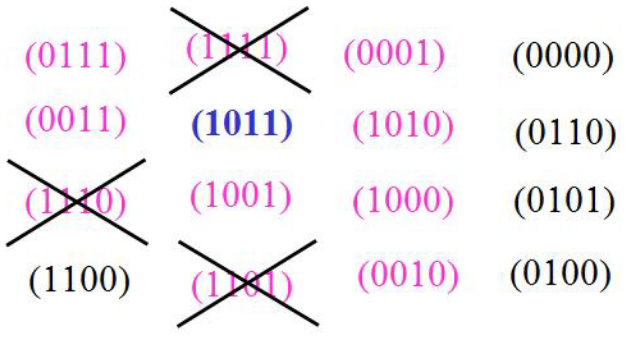
\includegraphics[width=0.6\columnwidth]{img/KPN1}
\end{center}

since subsets $\{1, 2, 3, 4\}, \{1, 2, 3\}$ and $\{1, 2, 4\}$ are unfeasible.\\

$10$ subsets (pink) have Hamming distance $\leq 2$ from $x = \{1, 3, 4\}$ (blue).\\

The neighborhood $N_{H_2} (x)$ consists of the $7$ feasible subsets in pink.\\
$N_{H_2} (x)$ excludes
\begin{itemize}
	\item the $3$ crossed subsets in pink because they are unfeasible
	
	\item the $5$ subsets in black because their Hamming distance from $x$ is $> 2$
\end{itemize}

The neighborhood must include only feasible solutions which respect the Hamming distance.\\

\newpage

\subsubsection{Neighborhoods based on operations}

Another common definition of neighborhood is obtained defining
\begin{itemize}
	\item a \textbf{family} $\mathcal{O}$ \textbf{of operations} on the solutions of the problem
	
	\item the \textbf{set of all solutions generated applying to} $x$ \textbf{the operations of} $\mathcal{O}$
	$$ N_{\mathcal{O}} (x) = \left\{x' \in X : \, \exists o \in \mathcal{O}: \, o (x) = x' \right\} $$
\end{itemize}

Considering again the KP, $\mathcal{O}$ can be defined as
\begin{itemize}
	\item \textbf{adding} to $x$ an element of $B \setminus x$
	
	\item \textbf{deleting} from $x$ at most an element (just to impose $x \in N (x)$)
	
	\item \textbf{swapping} one element of $x$ with one of $B \setminus x$
\end{itemize}

The resulting neighborhood $N_{\mathcal{O}}$ is related to those defined by the Hamming distance, but does not coincide with any of them
$$ N_{H_1} \subset N_{\mathcal{O}} \subset N_{H_2} $$
The Hamming distance 1 is just one operation, with this definition we can do more stuff, so it's bigger.\\

As the distance-based ones, these \textbf{neighborhoods can be parameterized} considering \textbf{sequences of} $k$ \textbf{operations} of $\mathcal{O}$ instead of a single one
$$ N_{\mathcal{O}_k} (x) = \left\{ x' \in X : \, \exists o_1, \, ... \, , o_k \in \mathcal{O} : \, o_k (o_{k-1} ( \, ... \, o_1 (x))) = x' \right\} $$ 
(bunch of operations, one after the other).\\

Essentially, define what you can do on a set (operations), and set a "number of operations away" distance metric.\\	

\newpage

\subsubsection{Distance and operation-based}

In general, an \textbf{operation-based} neighborhood includes solutions with \textbf{different Hamming distances from} $x$.\\

For the TSP one can define a neighborhood $N_{\mathcal{S}_1}$ including the solutions obtained swapping two nodes in their visit order

\begin{center}
	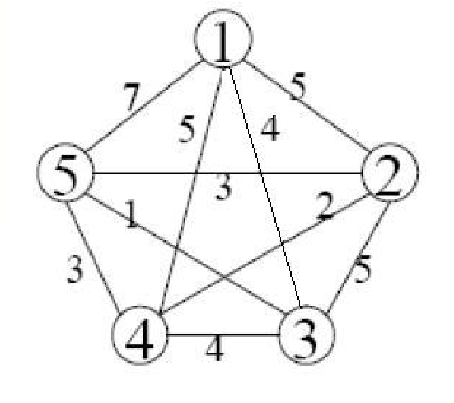
\includegraphics[width=0.5\columnwidth]{img/TSP2}
\end{center}

The neighborhood of solution $x = (3, 1, 4, 5, 2)$ is ($5$ vertices so $(5 \cdot 4) / 2$ pairs):
$$ \begin{array}{c c}
	N_{\mathcal{S}_1} (x) = & \{({\color{red} 1}, {\color{red} 3}, 4, 5, 2) , ({\color{red} 4}, 1, {\color{red} 3}, 5, 2) , ({\color{red} 5}, 1, 4, {\color{red} 3}, 2) , ({\color{red} 2}, 1, 4, 5, {\color{red} 3}) , (3, {\color{red} 4}, {\color{red} 1}, 5, 2) , \\
	& (3, {\color{red} 5}, 4, {\color{red} 1}, 2) , (3, {\color{red} 2}, 4, 5, {\color{red} 1}) , (3, 1, {\color{red} 5}, {\color{red} 4}, 2) , (3, 1, {\color{red} 2}, 5, {\color{red} 4}) , (3, 1, 4, {\color{red} 2}, {\color{red} 5}) \}
\end{array} $$
If the two nodes are adjacent, the modified arcs are $3 + 3$; otherwise, they are $4 + 4$.\\

This neighborhood cannot be defined as one with Hamming distance, in this case for this solution you include $4$ arcs less and $4$ more (to make the swap), $3$ if the node were adjacent, so the Hamming distance between two of these solutions would be $8$, $6$ in the case of adjacent nodes.\\
We can see that this neighborhood doesn't coincide with $N_{H_8}$ nor with $N_{H_6}$.\\

\newpage

\paragraph{Relations:} Sometimes the two definitions yield the same neighborhood
\begin{itemize}
	\item for the MDP
	\begin{itemize}
		\item $N_{H_2}$ (solutions at Hamming distance equal to $2$)
		\item $N_{\mathcal{S}_1}$ (swap one element of $x$ with one of $B \setminus x$)
	\end{itemize}
	\nn
	
	\item for the BPP
	\begin{itemize}
		\item $N_{H_2}$ (solutions at Hamming distance equal to $2$)
		\item $N_{\mathcal{T}_1}$ (transfer an object into a different container)
	\end{itemize}
	\nn
	
	\item for Max-SAT
	\begin{itemize}
		\item $N_{H_2}$ (solutions at Hamming distance equal to $2$)
		\item $N_{\mathcal{F}_1}$ ("flip" a variable: invert its truth assignment)
	\end{itemize}
	\nn
\end{itemize}

This is typical of problems with \textbf{solutions of fixed cardinality}:
\begin{itemize}
	\item perform a \textbf{sequence of} $k$ swaps between single elements $(|A| = |D| = 1)$: $k$ elements go into $x$ and $k$ elements go out
	
	\nn
	
	\item the \textbf{Hamming distance} between the two extreme solutions \textbf{is} $\leq 2k$ (if all exchanged elements are different, it is exactly $2k$)
\end{itemize}

\newpage

\paragraph{Different neighborhoods for the same problem:} the CMST.\\

Different ground sets yield different neighborhoods. In the CMST it is possible to set $B = E$ or $B = V \times T$
\begin{itemize}
	\item exchange \textbf{edges}: delete $(b, c)$, add $(b, e)$
	\begin{center}
		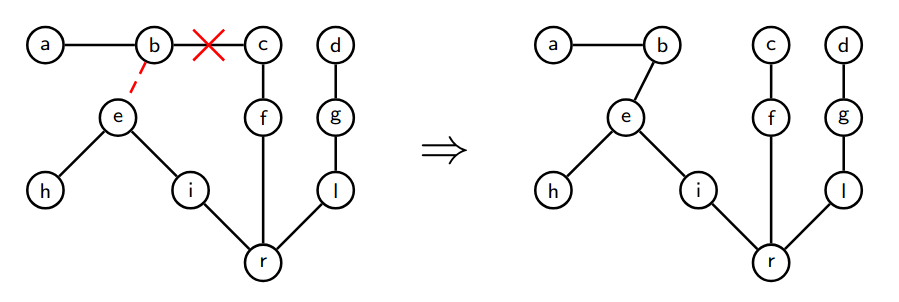
\includegraphics[width=0.85\columnwidth]{img/CMST1}
	\end{center}
	\nn
	
	\item exchange \textbf{vertices}: move $e$ from subtree 2 to subtree 1, and recompute the two minimum spanning subtrees
	\begin{center}
		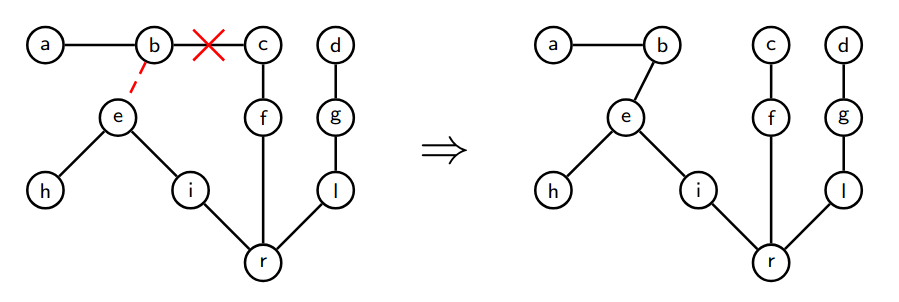
\includegraphics[width=0.85\columnwidth]{img/CMST1}
	\end{center}
\end{itemize}

\newpage

\textbf{PSMP:} For the PMSP it is possible to define
\begin{itemize}
	\item the transfer neighborhood $N_{\mathcal{T}_1}$, based on the set $\mathcal{T}_1$ of \textbf{all transfers} of a task on another machine
	\begin{center}
		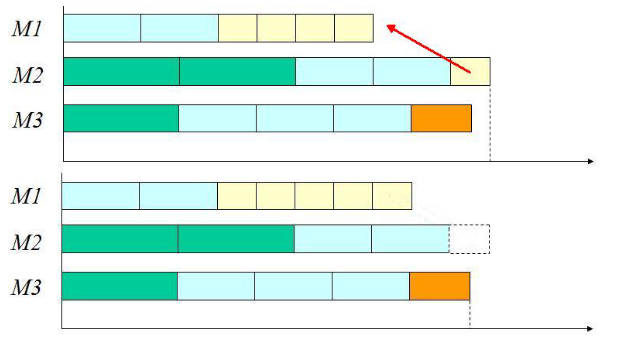
\includegraphics[width=0.7\columnwidth]{img/PSMP1}
	\end{center}
	\nn
	
	\item the swap neighborhood $N_{\mathcal{S}_1}$, based on the set $\mathcal{S}_1$ of the \textbf{swaps of two tasks} between two machines (one task for each machine)
	\begin{center}
		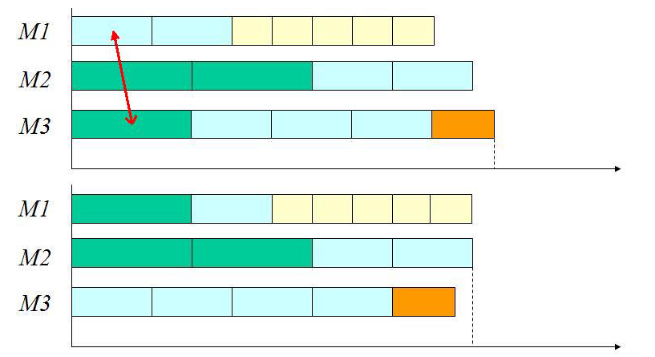
\includegraphics[width=0.7\columnwidth]{img/PSMP2}
	\end{center}
	\nn
\end{itemize}

\newpage

\subsubsection{Connectivity of the search graph}

An exchange heuristic can return the optimum only if \textbf{every feasible solution} can \textbf{reach} at least \textbf{one optimal solution}, that is there is a path from $x$ to $X^\ast$ for every $x \in X$.\\

Such a search graph is denoted as \textbf{weakly connected} to the optimum.\\

Since $X^\ast$ is unknown, a \textbf{stronger condition} is often used: a search graph is \textbf{strongly connected} when it admits a path from $x$ to $y$ for every $x, y \in X$.\\

A \textbf{good neighborhood} should guarantee some \textbf{connectivity conditions}
\begin{itemize}
	\item in the MDP, neighborhood $N_{\mathcal{S}_1}$ connects any pair of solutions with at most $k$ swaps
	
	\item in the KP and the SCP, no neighborhood $N_{\mathcal{S}_k}$ gives that guarantee (feasible solutions can have any cardinality)
	
	\item the search graph becomes connected also in the KP and the SCP if swaps are combined with both additions and deletions
\end{itemize}

Strong connectivity is when every feasible solution is reachable from every other feasible solution. Everything is connected.\\

If feasibility is defined in a sophisticated way, exchanging, adding and deleting \textbf{single} elements can be \textbf{insufficient} to reach all solutions: the \textbf{unfeasible subsets} can \textbf{break} all \textbf{paths} between some feasible solutions.

\begin{center}
	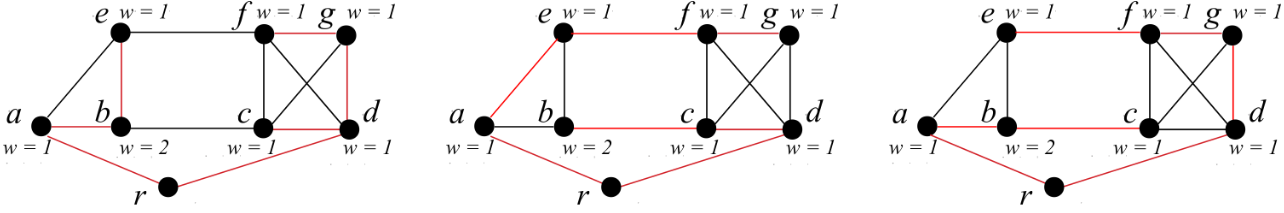
\includegraphics[width=\columnwidth]{img/connectivity}
\end{center}

If $V = 4$, only three solutions are feasible, all with two subtrees:
$$
\begin{array}{c c}
	x & = \{(r , a) , (a, b) , (b, e) , (r , d) , (c, d) , (d, g ) , (f , g )\} \\
	x' & = \{(r , a) , (a, e) , (e, f ) , (r , d) , (c, d) , (b, c) , (f , g )\} \\
	x'' & = \{(r , a) , (a, b) , (e, f ) , (r , d) , (b, c) , (d, g ) , (f , g )\}
\end{array}
$$
The three solutions are mutually reachable only exchanging at least two edges at at time; exchanging only one yields unfeasible subsets.

\newpage

\subsection{Steepest descent (hill-climbing) heuristics}
Abandoning the concept of neighborhood, let's consider how to move within them, what is the selection criteria?\\

The \textbf{simplest selection criteria} $\varphi (x, A, D)$ is the \textbf{objective function} (it is used in nearly all exchange heuristics).\\

\textbf{When} $\varphi (x, A, D) = f (x \cup A \setminus D)$, the \textbf{heuristic moves from} $x^{(t)}$ \textbf{to} the best solution in $N (x^{(t)})$ (this is considering only the update in value, not recalculating the whole objective function, if it makes the computation easier).\\

To avoid cyclic behavior, \textbf{only strictly improving solutions} are accepted. You can't "go back", otherwise you risk visiting multiple times the same solutions (if an earlier solution was better why not going back to it?).\\
Consequently, \textbf{the best known solution is the last visited one}.\\

Steepest \textit{Descent} for minimization, \textit{Ascent/Hill-climbing} for maximization.
\begin{algorithm}
	\caption{Algorithm $SteepestDescent(I , x^{(0)})$}
	\begin{algorithmic}
		\STATE $x := x^{(0)}$
		\STATE Stop$ := false$
		\WHILE{Stop$=false$}
		\STATE $\overline{x} := \arg \min_{x' \in N(x)} f(x')$
		\IF{$f(\overline{x}) \geq f(x)$}
		\STATE Stop$ := true$
		\ELSE 
		\STATE $x := \overline{x}$
		\ENDIF
		\ENDWHILE
		\RETURN $(x, f (x))$
	\end{algorithmic}
\end{algorithm}
Note that the best solution is not saved, since it's always the last one.\\

\newpage

\subsubsection{Local and global optimality}
A steepest descent heuristic \textbf{terminates}, by definition, when it finds a \textbf{locally optimal solution}, that is a solution $\overline{x} \in X$ such that
$$ f (\overline{x}) \leq f (x) \text{ for each } x \in N (x) $$
A local optimum is the best (technically not worse) solution inside of a neighborhood. 

\begin{center}
	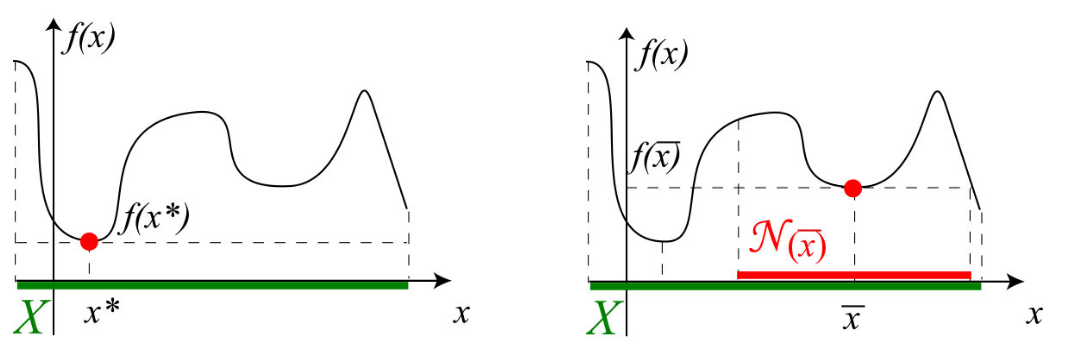
\includegraphics[width=\columnwidth]{img/localOptimum}
\end{center}

A globally optimal solution is always also locally optimal, but the opposite is not true in general: $X^\ast \subseteq \overline{X}_N \subseteq X$.\\

There could be a better solution outside of the neighborhood, so the set of locally optimal solution is dependent on the definition of neighborhood.\\

\newpage

\subsubsection{Exact neighborhood}

\textbf{Exact neighborhood} is a neighborhood function $N : \, X \rightarrow 2^X$ such that \textbf{each local optimum is also a global optimum}
$$ \overline{X}_N = X^\ast $$

\textbf{Trivial case:} the neighborhood of each solution coincides with the whole feasible region ($N (x) = X$ for each $x \in X$, if I have the whole set I'm going to get the optimum). It's a useless neighborhood: too wide to explore.\\

The exact neighborhoods are \textbf{extremely rare}; examples: 
\begin{itemize}
	\item exchange between edges for the Minimum Spanning Tree problem
	
	\item exchange between basic and nonbasic variables used by the simplex algorithm for Linear Programming
\end{itemize}

In general, the steepest descent heuristic does not find a global optimum.\\

Its effectiveness depends on the properties of search graph and objective.\\

Essentially is a neighborhood that includes the global optimum; in general it's hard to obtain.\\

\newpage

\subsubsection{Properties of the search graph}
The properties of the graph can determine if our algorithm will find a "good" local optimum or a "bad" local optimum.\\

Some relevant properties for the effectiveness of an algorithm are
\begin{itemize}
	\item The \textbf{size of the search space} $|X|$ (big space needs big time, small space needs small time).\\
	
	\item The \textbf{connectivity of the search graph} (as discussed above, maybe the optimal solution is in a not connected part of the graph).\\
	
	\item The \textbf{diameter of the search graph}, that is the number of arcs of the minimum path between the two farthest solutions: larger neighborhoods produce graphs of smaller diameter (but other factors exist: see the "smallworld" effect).\\
\end{itemize}
\nn

Consider neighborhood $N_{\mathcal{S}_1}$ for the symmetric TSP on complete graphs
\begin{itemize}
	\item the search space includes $|X| = (n − 1)!$ solutions
	
	\item $N_{\mathcal{S}_1}$ (swap of two nodes) includes $\left(\begin{array}{c}
		n \\ 2 \end{array}\right) = n(n-1)/2$ solutions
	
	\item the search graph is strongly connected and has diameter $\leq n - 2$: every solution turns into another after at most $n - 2$ swaps.\\
	For example, $x = (1, 5, 4, 2, 3)$ becomes $x' = (1, 2, 3, 4, 5)$ in $3$ steps
	$$ x = (1, 5, 4, 2, 3) \rightarrow (1, 2, 4, 5, 3) \rightarrow (1, 2, 3, 5, 4) \rightarrow (1, 2, 3, 4, 5) = x' $$
	(the first node is always $1$, the last one is automatically in place)
\end{itemize}

\newpage

Other \textbf{relevant properties}:
\begin{itemize}
	\item The \textbf{density of global optima} $( |X^\ast|/|X |)$ \textbf{and local optima} $( | \overline{X}_N | / |X | )$: if the local optima are numerous, it is hard to find the global ones. \\
	How many global and local optima you have versus the total number of solutions. \\
	
	\item The \textbf{distribution of the quality} $\delta (\overline{x})$ \textbf{of local optima} (SQD diagram): if local optima are good, it is less important to find a global one. \\
	
	\item The \textbf{distribution of the locally optimal solutions in the search space}: if local optima are close to each other, it is not necessary to explore the whole space.\\
\end{itemize}

These indices would require an exhaustive exploration of the search graph.\\

In pratice, one performs a sampling and these analyses
\begin{itemize}
	\item require very long times
	\item can be misleading, especially if the global optima are unknown
\end{itemize}

\newpage

\paragraph{Example:} the TSP. For the TSP on a complete symmetric graph with Euclidean costs
\begin{itemize}
	\item The Hamming distance between two local optima is on average $\ll n$: the local optima concentrate in a small region of $X$.\\
	
	\item The Hamming distance between local optima on average exceeds that between local and global optima: the global optima tend to concentrate in the middle of local optima.\\
	
	\item The \textit{FDC} diagram (Fitness-Distance Correlation) reports the quality $\delta (\overline{x})$ versus the distance from global optima $d_H (\overline{x}, X^\ast)$ (for each local optima, on the horizontal axis is shown how far they are from the global, on the vertical axis there's the percentage deviation $\delta$): if they are correlated, better local optima are closer to the global ones.\\
\end{itemize}
\begin{center}
	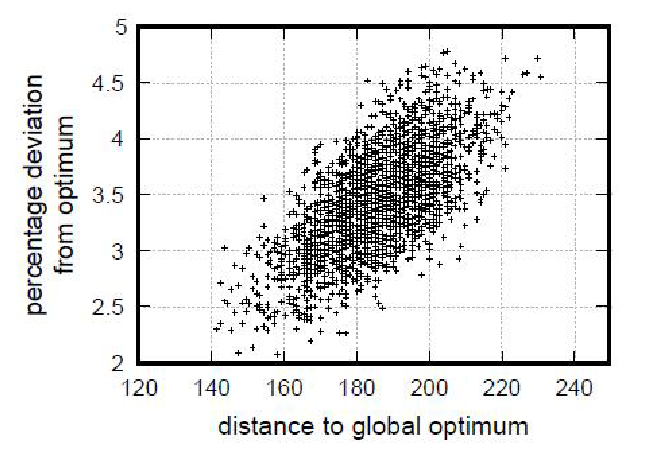
\includegraphics[width=0.7\columnwidth]{img/TSP3}
\end{center}

This diagram teaches that if, after you found a local optimum, it's good to (somehow) continue and intensify the search because you will probably move towards the global optimum.\\

\newpage

For the Quadratic Assignment Problem (QAP), the situation is different
\begin{center}
	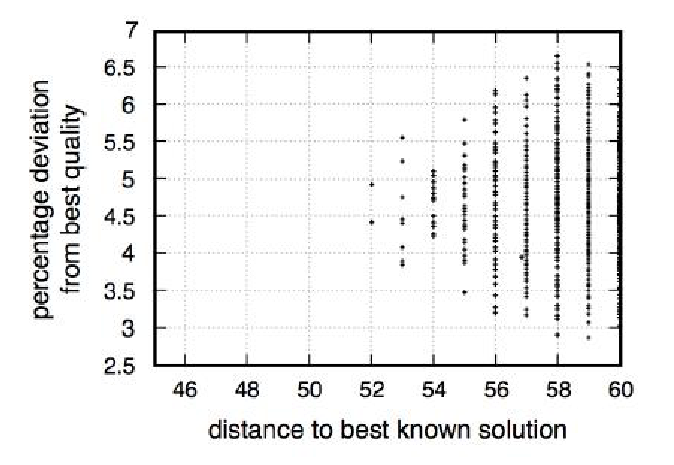
\includegraphics[width=0.7\columnwidth]{img/QAP}
\end{center}

If \textbf{quality} and \textbf{closeness} to the global optima are \textbf{strongly correlated}
\begin{itemize}
	\item It is \textbf{profitable} to \textbf{build good starting solutions}, because they drive the search near a good local optimum.\\
	
	\item It is \textbf{better} to \textbf{intensify} than to diversify.\\
\end{itemize}

If the \textbf{correlation is weak}
\begin{itemize}
	\item A good \textbf{initialization is less important}.\\
	
	\item It is \textbf{better} to \textbf{diversify} than to intensify
\end{itemize}

\newpage

\subsection{Landscape}
The \textbf{landscape} is the \textbf{triplet} $(X , N, f )$, where
\begin{itemize}
	\item $X$ is the \textbf{search space}, or the set of feasible solutions
	
	\item $N : X \rightarrow 2^X$ is the \textbf{neighborhood function}
	
	\item $f : X \rightarrow \mathbb{N}$ is the \textbf{objective function}
\end{itemize}

It is the \textbf{search graph with node weights given by the objective}. The first two terms correspond to the search graph, the last one gives weights to the nodes.\\

The \textbf{effectiveness} of steepest descent \textbf{depends} on the \textbf{landscape}
\begin{itemize}
	\item \textbf{smooth landscapes} yield few local optima, possibly of good quality, hence to \textbf{good results}
	
	\item \textbf{rugged landscapes} yield several local optima of widespread quality, hence to \textbf{bad results}
\end{itemize}

There is a \textbf{great variety of landscapes}, very different from one another
\begin{center}
	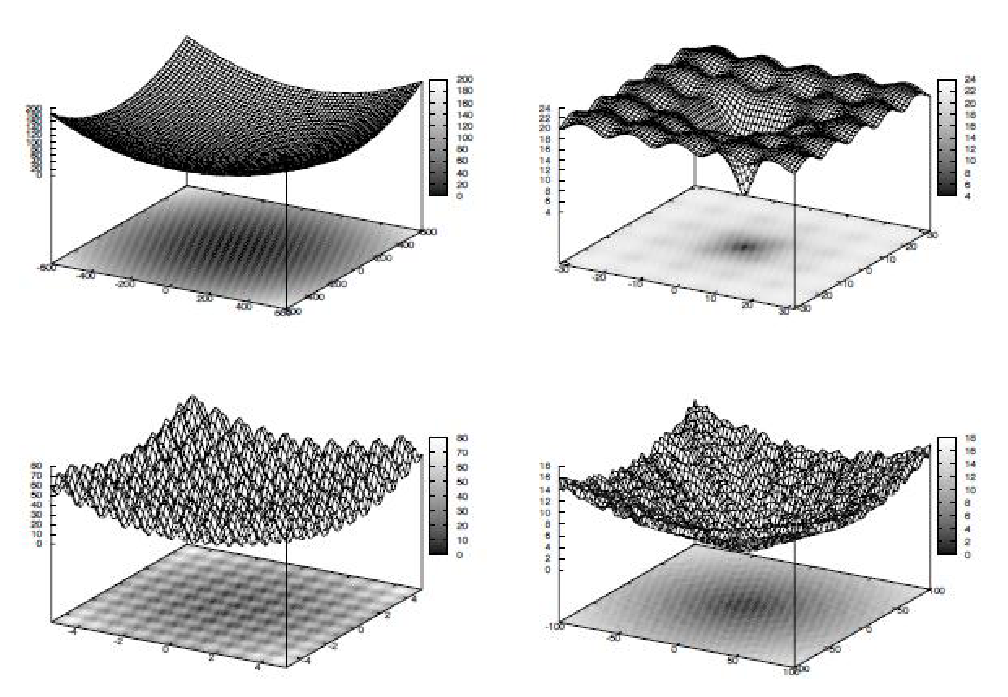
\includegraphics[width=0.9\columnwidth]{img/landscape1}
\end{center}

\newpage

\subsubsection{Autocorrelation coefficient}
The \textbf{complexity of a landscape} can be \textbf{empirically estimated}
\begin{enumerate}
	\item performing a \textbf{random walk} in the \textbf{search graph}
	
	\item determining the \textbf{sequence} of \textbf{values} of the \textbf{objective} $f^{(1)}, \, ... \, , f^{(t_{max})}$
	
	\item computing the \textbf{sample mean} 
	$$ \overline{f} = \frac{\displaystyle \sum_{t=1}^{t_{max}} f^{(t)}}{\displaystyle t_{max}} $$
	
	\item computing the \textbf{empirical autocorrelation coefficient}
	$$ r(i) = \frac{\displaystyle \frac{\displaystyle \sum_{t=1}^{t_{max} - i} \left(f^{(t)} - \overline{f}\right) \left(f^{(t+i)} - \overline{f}\right) }{\displaystyle t_{max} - i } }{\displaystyle \frac{\displaystyle \sum_{t=1}^{t_{max}} \left(f^{(t)} - \overline{f}\right)^2 }{\displaystyle t_{max} }}$$
	This is trying to relate the values of the objective function to the mean, with the goal of understanding how much these values vary; the denominator is the mean square error; the numerator is trying to know the difference between a step and the next, that way it can describe if the landscape is a smooth curve or a really rugged one (both could differ the same from the mean)
\end{enumerate}
That \textbf{relates} the \textbf{difference of the objective values in the solutions visited} with the \textbf{distance between these solutions along the walk}.\\

This is trying to give a function to describe the "ruggedness" of a landscape.\\

\newpage

Idea is:
\begin{itemize}
	\item With $i=0 \rightarrow r (0) = 1$ (perfect correlation at $0$ distance); numerator and denominator are the same, increasing the $i$ is considering "how much is the value changing?".\\
	
	\item In general $r (i)$ \textbf{decreases} as the \textbf{distance} $i$ \textbf{increases}.\\
	
	\item \textbf{If} $r (i) \approx 1$ in a large range of distances, the \textbf{landscape is smooth}:
	\begin{itemize}
		\item the neighbor solutions have values close to the current one
		\item there are few local optima
		\item the steepest descent heuristic is effective
	\end{itemize}
	\nn
	
	\item \textbf{If} $r (i)$ \textbf{varies steeply}, the \textbf{landscape is rugged}:
	\begin{itemize}
		\item the neighbor solutions have values far from the current one
		\item there are many local optima
		\item the steepest descent heuristic is ineffective
	\end{itemize}
	\nn
\end{itemize}

\newpage

\subsubsection{Plateau}
The \textbf{search graph} can be \textbf{partitioned} according to the \textbf{objective value}
\begin{itemize}
	\item \textbf{plateau of value} $f$ is each subset of solutions of value $f$ that are adjacent in the search graph (a bunch of equal values together)
\end{itemize}
\begin{center}
	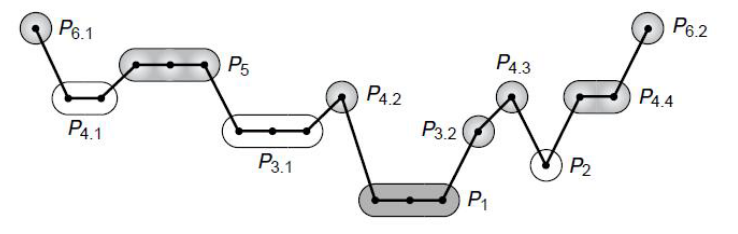
\includegraphics[width=0.7\columnwidth]{img/plateau1}
\end{center}

\textbf{Large plateaus complicate the choice of the solution}: most neighbors are equivalent, and the choice ends up depending on the visit order. An extremely uniform landscape is not an advantage.\\

Example: all transfers and swaps between machines 1 and 3 leave the objective value unchanged (most other moves worsen it)
\begin{center}
	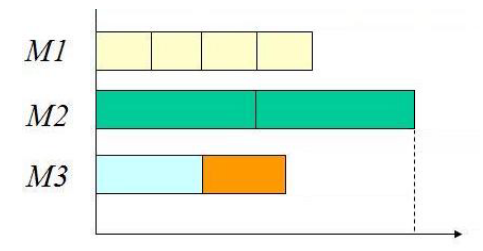
\includegraphics[width=0.55\columnwidth]{img/plateau2}
\end{center}

A plateau gives a lot of choices that are all effectively the same, making the objective function a bad criteria.\\

\newpage

\subsubsection{Attraction basins}
\textbf{Alternatively}, the \textbf{search graph} can be \textbf{partitioned} into:
\begin{itemize}
	\item \textbf{attraction basins} of the \textbf{locally optimal solutions} $\overline{x}$, that are the subsets of solutions $x^{(0)} \in X$ starting from which the steepest descent heuristic terminates in $\overline{x}$ (if I start with a steepest descent in the basin, I'm going to get $x$ since it's the closest local optimum)
\end{itemize}
\begin{center}
	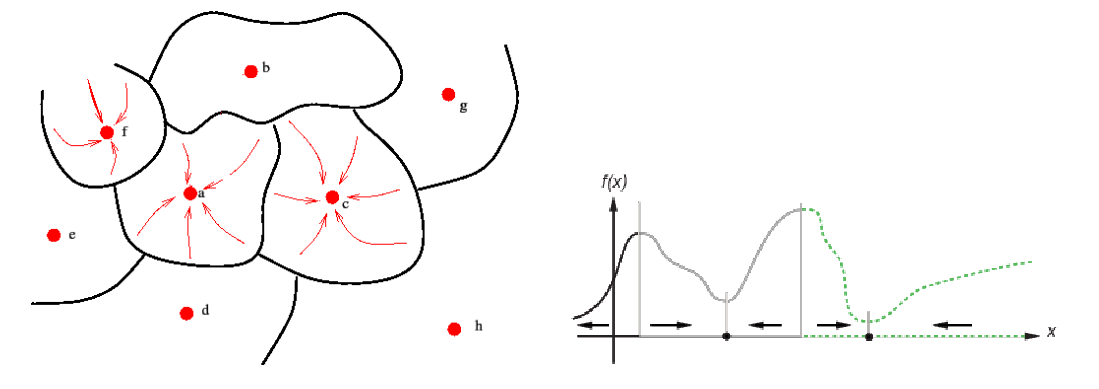
\includegraphics[width=\columnwidth]{img/basins}
\end{center}
The basins are separated by frontiers, on one side I get a local optimum, on the other side I get a different local optimum.\\ 

The steepest descent heuristic is
\begin{itemize}
	\item \textbf{Effective} if the attraction \textbf{basins} are \textbf{few and large} (especially if the global optima have larger basins), even if the algorithm will have to take a lot of steps.\\
	
	\item \textbf{Ineffective} if the attraction \textbf{basins} are \textbf{many and small} (especially if the global optima have smaller basins).\\
\end{itemize}

% End of L13

\newpage

\subsection{Complexity}
The complexity of the steepest descent heuristic depends on
\begin{itemize}
	\item The \textbf{number of iterations} $t_{max}$ \textbf{from} $x^{(0)}$ \textbf{to the local optimum found}, which depends on the structure of the search graph (width of the attraction basins) and is hard to estimate a priori.\\
	
	\item The \textbf{search for the best solution in the neighborhood} $(\overline{x})$, which depends on how the search itself is performed, but whose complexity estimation is usually standard.\\
\end{itemize}

\subsubsection{The exploration of the neighborhood}
It's the function in which you minimize the value of the objective.\\

\textbf{Two strategies} to explore the neighborhood are possible
\begin{enumerate}
	\item \textbf{Exhaustive search:} evaluate \textbf{all the neighbor solutions}; the complexity of a single step is the product of
	\begin{itemize}
		\item the number of neighbor solutions $(|N (x)|)$
		\item the evaluation of the cost of each solution $(\gamma_f (|B|, x))$
	\end{itemize}
	If it is not possible to generate only feasible solution:
	\begin{itemize}
		\item visit a superset of the neighborhood $( \tilde{N} (x) \supset N (x))$
		\item for each element $x$, evaluate the feasibility $(\gamma_X (|B|, x))$
		\item for the feasible ones, evaluate the cost $(\gamma_f (|B|, x))$
	\end{itemize}
	\nn
	
	\item \textbf{Efficient exploration} of the neighborhood \textbf{without a complete visit:} find the \textbf{best neighbor solution solving an auxiliary problem}. Only some special neighborhoods allow that.\\
\end{enumerate}

\newpage

\paragraph{Exhaustive visit of the neighborhood} \nn

\begin{algorithm}
	\caption{Algorithm $SteepestDescent(I , x^{(0)})$}
	\begin{algorithmic}
		\STATE $x := x^{(0)}$
		\STATE Stop $:= false$
		\WHILE{Stop $= false$}
		\STATE $ \tilde{x} := x$ // $\tilde{x} := \arg \min_{x' \in N(x)} f(x')$
		\FOR{each $x' \in \tilde{N}$}
		\IF{$x' \in N(x)$}
		\IF{$f(x') < f(\tilde{x})$}
		\STATE $\tilde{x} := x'$
		\ENDIF
		\ENDIF
		\ENDFOR
		\IF{$f(x') \geq f(x)$}
		\STATE Stop $ := true$
		\ELSE
		\STATE $x := \tilde{x}$
		\ENDIF
		\ENDWHILE
		\RETURN $(x, f (x))$
	\end{algorithmic}
\end{algorithm}

The \textbf{complexity} of the neighborhood exploration \textbf{combines} three terms
\begin{enumerate}
	\item $| \tilde{N} (x) |$: the \textbf{number of subsets visited}.\\
	
	\item $\gamma_X$: the \textbf{time to evaluate their feasibility}.\\
	
	\item $\gamma_f$: the \textbf{time to evaluate the objective} for a feasible solution.\\
\end{enumerate}

\newpage

\subsubsection{Evaluating or updating the objective}

\paragraph{The additive case:} The first way to accelerate an exchange algorithm is to \textbf{minimize the time to evaluate the objective}: in particular, it is \textbf{faster} to \textbf{update} $f (x)$ rather \textbf{than to recompute} it.\\

The \textbf{update of an additive objective} $f (x) = \sum_{j \in x} \phi_j$ requires to
\begin{itemize}
	\item Sum $\phi_i$ for each element $i \in A$, added to $x$.\\
	
	\item Subtract $\phi_j$ for each element $j \in D$, deleted from $x$
	$$ \delta f (x, A, D) = f (x \cup A \setminus D) - f(x) = \sum_{i \in A} \phi_i - \sum_{j \in D} \phi_j $$
	\nn
\end{itemize}

Examples: swap of objects (KP), columns (SCP), edges (CMSTP), ...\\

This \textbf{update} has \textbf{two} fundamental \textbf{properties}:
\begin{itemize}
	\item It takes \textbf{constant time for a constant number of elements} $|A| + |D|$.\\
	
	\item $\delta f (x, A, D)$ \textbf{does not depend on} $x$ (only on the elements added and deleted, more about it later).\\
\end{itemize}

If the objective function is additive just add and subtract the changes.\\

\newpage

\paragraph{The quadratic case:} The MDP has a quadratic objective function: computing it costs $\Theta (n^2)$.\\

Moving from $x$ to $x' = x \setminus \{i\} \cup \{j\}$ (neighborhood $N_{\mathcal{S}_1}$, just making a swap), the \textbf{update is}
$$ \delta f (x,i,j) = f \left(x \setminus \left\{i\right\} \cup \left\{j\right\}\right) - f(x) = \sum_{h,k \in x \setminus \left\{i\right\} \cup \left\{j\right\}} d_{hk} - \sum_{h,k \in x} d_{hk} $$

Which \textbf{depends on} $O (n)$ distance terms, related to points $i$ and $j$ (everything else cancels out).\\

There is a general trick \textbf{for the symmetric quadratic functions} with $d_{ii} = 0$

$$ \delta f (x,i,j) = \sum_{h \in x \setminus \left\{i\right\} \cup \left\{j\right\}} \; \sum_{k \in x \setminus \left\{i\right\} \cup \left\{j\right\}} d_{hk} - \sum_{h \in x} \; \sum_{k \in x} d_{hk} \implies $$
$$ \implies \delta f (x,i,j) = 2 \sum_{k \in x} d_{jk} - 2 \sum_{k \in x} d_{ik} - 2 d_{ij} = 2 \left(D_j (x) - D_i (x) - d_{ij}\right) $$

If $D_{\ell} (x) = \sum_{k \in x} d_{\ell k}$ is known for each $\ell \in B$, \textbf{the computation takes} $O (1)$.\\

If you save the distance from every element to the solution (distance from every other element in the solution set) there's no need to calculate $D_j (x)$ and $D_i (x)$ (distance from point $j$ and $i$ to the solution) every time, leaving out only $d_{ij}$, which has to be subtracted (since we don't have $i$ anymore) and can be done in constant time.\\

From the objective function we just need to add the distances relative to $j$ (represented in $D_j (x)$), subtract the distances from $i$ to the other elements in the solution ($D_i (x)$), and also subtract the distance from $j$ to $i$, since $i$ is not in the solution anymore. If we keep an auxiliary data structure for the distances $D_{\ell} (x)$ for every $\ell \in x$ then this update takes constant time. The auxiliary structures will have to be updated in $O (n)$ time each iteration. \\

\newpage


Example: the MDP
\begin{center}
	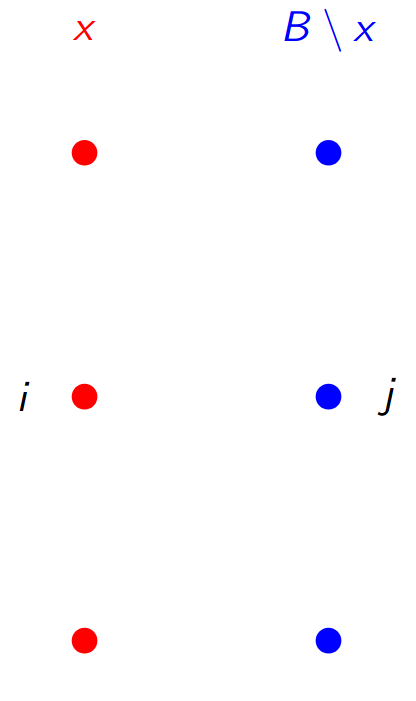
\includegraphics[width=0.25\columnwidth]{img/MDP2}
\end{center}
Let us consider $f (x) /2$.\\

Evaluate the exchange
$$ x \rightarrow x' = x \setminus \{i\} \cup \{j\} $$
with $i \in x$ and $j \in B \setminus x$ (swapping $i$ from the solution with $j$ from outside, $i$ becomes blue, $j$ becomes red).\\

$$ f (x') = f (x) − D_i + D_j − d_{ij} $$

\begin{itemize}
	\item the pairs including $i$ are lost
	\item the pairs including $j$ are acquired
	\item but the pair $(i, j)$ is in excess
\end{itemize}
The cost is computed in $O (1)$ time for each solution.\\

\textbf{Update of the data structures}:
$$ D_{\ell} = D_{\ell} - d_{\ll i} + d_{\ell j} \;\;\; \ell \in B $$
For each element $\ell \in B$
\begin{itemize}
	\item $d_{\ll i}$ disappears
	\item $d_{\ell j}$ appears
\end{itemize}

The auxiliary data structure is updated in $O (n)$ time for each iteration.\\

\newpage

\paragraph{Nonlinear examples:} Many nonlinear functions can be updated with similar tricks
\begin{itemize}
	\item save aggregated information on the current solution $x^{(t)}$
	
	\item use it to compute $f (x')$ efficiently for each $x' \in N (x^{(t)})$
	
	\item update it when moving to the following solution $x^{(t+1)}$
\end{itemize}

Using the transfer ($N_{\mathcal{T}_1}$) and swap ($N_{\mathcal{S}_1}$) neighborhoods for the PMSP, the objective can be updated in constant time by managing
\begin{enumerate}
	\item the completion time for each machine
	
	\item the indices of the machines with the first and second maximum time
\end{enumerate}

\begin{center}
	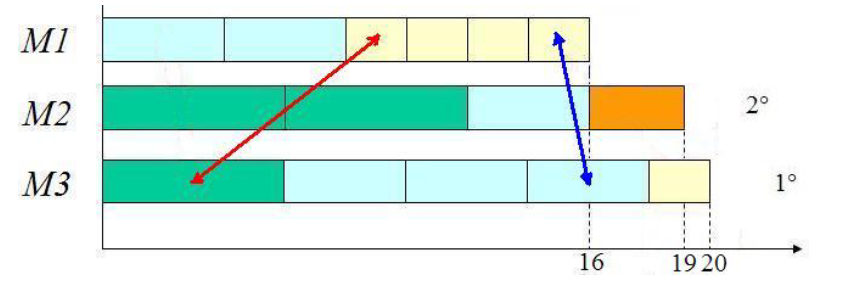
\includegraphics[width=0.75\columnwidth]{img/PMSP2}
\end{center}

Consider the swap $o = (i, j)$ of tasks $i$ and $j$ ($i$ on machine $M_i$, $j$ on machine $M_j$)
\begin{itemize}
	\item compute in constant time the new completion times: one increases, the other decreases (or both remain constant)
	
	\item test in constant time whether either exceeds the maximum
	
	\item if the maximum time decreases, test in constant time whether the other time or the second maximum time becomes the maximum
\end{itemize}

Once the neighborhood is visited and the exchange selected, update
\begin{itemize}
	\item the two modified completion times (each one in constant time)
	
	\item their positions in a max-heap (each one in time $O (\log |M|)$)
\end{itemize}
\nn	

Basically, compute the new the times, check if there's a new maximum, check if the maximum is still the maximum (if needed), then update the data structures. \\

To do this we need to remember: completion time for each machine and which machines have the maximum and the second maximum time.

\newpage

\paragraph{Use of local auxiliary information:} The auxiliary information used to compute $f (x')$ can be
\begin{itemize}
	\item \textbf{global}, that is referring to the \textbf{current solution} $x$
	
	\item \textbf{local}, that is referring to the \textbf{solution} $p_N (x')$ \textbf{visited before} $x'$ in neighborhood $N (x)$ according to a suitable order
\end{itemize}

Consider the neighborhood $N_{\mathcal{R}_2}$ for the asymmetric TSP:
\begin{itemize}
	\item the neighbor solutions differ from $x$ for $O (n)$ arcs
	
	\item general neighbor solutions differ from each other for $O (n)$ arcs
	
	\item if the pairs of arcs $(s_i , s_{i+1})$ and $(s_j , s_{j+1})$ follow the lexicographic order, the reverted path changes only by one arc
\end{itemize}

\begin{center}
	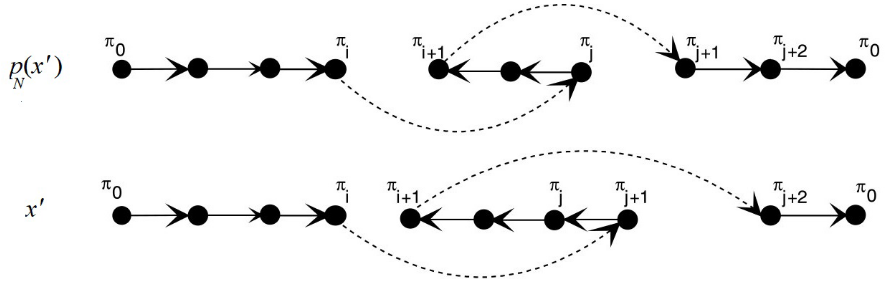
\includegraphics[width=0.9\columnwidth]{img/TSP4}
\end{center}

The \textbf{variation} of $f (x)$ between \textbf{two generic neighbor} solutions is
$$ \delta f (x, i, j) = c_{s_i ,s_j} + c_{s_{i+1}, s_{j+1}} - c_{s_i ,s_{i+1}} - c_{s_j ,s_{j+1}} + c_{s_j \, ... \, s_{i+1}} - c_{s_{i+1} \, ... \, s_j} $$

but moving from exchange $(s_i , s_j )$ to exchange $(s_i , s_{j+1})$
\begin{itemize}
	\item the first four terms change, but they can be checked in constant time
	
	\item the last two terms can be updated in constant time
	$$ \begin{cases}
		c_{s_{j'} \, ... \, s_{i+1}} & = c_{s_j \, ... \, s_{i+1}} + c_{s_{j+1},s_j} \\
		c_{s_{i+1} \, ... \, s_{j'}} & = c_{s_{i+1} \, ... \, s_j} + c_{s_j ,s_{j+1}}
	\end{cases}$$
\end{itemize}

Add the two arcs added (from $i$ to $j$ and from $i+1$ and $j+1$), remove the arcs that have been removed (from $i$ to $i+1$ and from $j$ to $j+1$), add the cost of the now reversed path, minus the cost of the original path. The last two terms (which can be big) can be updated in constant time by adding the new terms.\\
In constant time, with $6$ terms the function can be updated.\\

Is it acceptable to explore the neighborhood in a predefined order?

\newpage

\subsection{Feasibility of the neighborhood}
\textbf{Defining neighborhoods} with the Hamming distance or with operations \textbf{can generate} also \textbf{unfeasible subsets}, that \textbf{must be removed}

$$ \tilde{N}_{H_k} (x) = \{x' \subseteq B : \, d (x', x) \leq k \} \supseteq N_{H_k} (x) = \tilde{N}_{H_k} (x) \cap X $$

$$ \tilde{N}_{\mathcal{O}} (x) = \{ x' \subseteq B : \, \exists o \in \mathcal{O} : \, o (x) = x' \} \supseteq N_{\mathcal{O}} (x) = \tilde{N}_{\mathcal{O}} (x) \cap X $$

(Examples: KP, BPP, SCP, CMSTP ... ).\\

If it is not possible to avoid a priori the unfeasible subsets, one must
\begin{itemize}
	\item \textbf{Test} the \textbf{feasibility of each element} of $\tilde{N} (x)$ to obtain $N (x)$.\\
	
	\item For the feasible elements, \textbf{evaluate} the \textbf{cost}.\\
\end{itemize}

The feasibility test can be made efficient with techniques similar to the ones used for the objective evaluation.\\

Example: update in constant time the total volume of a subset in the KP.\\

\newpage

\paragraph{Example:} The CMSTP. Consider the swap neighborhood $N_{\mathcal{S}_1}$ (add one edge, delete another)
\begin{itemize}
	\item If the two edges are in the same branch, the solution remains feasible.\\
	
	\item If they are in different branches, one loses weight, the other acquires it: the variation is equal to the weight of the subtree transferred.\\
\end{itemize}

\begin{center}
	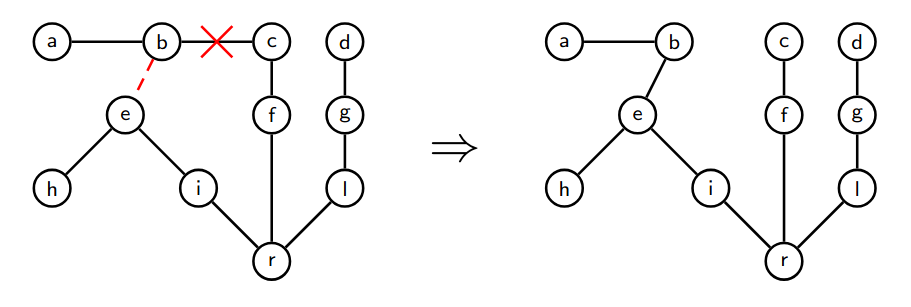
\includegraphics[width=0.8\columnwidth]{img/CMST3}
\end{center}

If each vertex saves the weight of its appended subtree, to test feasibility compare this weight with the residual capacity of the receiving branch (the weight appended to $b$ with the residual capacity of the left branch).\\

Once the best exchange is performed, the information must be updated in time $O (n)$ visiting the old ancestors from $c$ and the new ones from $e$.\\

If you know the total weight of the branch that has been cut (how many vertices are still appended) and confront that value with the residual capacity of the receiving branch.\\

You can save in a vector the total weight of the subtree appended to each vertex in the current solution. After a move you need to update all auxiliary information.\\

\newpage

\subsection{Partial saving of the neighborhood}

When performing an \textbf{operation} $o \in \mathcal{O}$ on a \textbf{solution} $x \in X$ sometimes
\begin{itemize}
	\item the \textbf{feasibility of the resulting solution} $o (x)$
	\item the \textbf{variation of the objective} $\delta f_o (x) = f (o(x)) − f (x)$
\end{itemize}
\textbf{depend only on a part of} $x$ (possibly, very small).\\

For example, consider the swap neighborhood $N_{\mathcal{S}_1}$ for the CMST:
\begin{itemize}
	\item add an edge $k \in B \setminus x$
	\item delete an edge $h \in x$
\end{itemize}
Two branches are involved: one acquires a subtree, the other loses it.\\

The \textbf{feasibility of swap} $(i, j)$ \textbf{depends} on the \textbf{branches including} $i$ \textbf{and} $j$: it is the \textbf{same in} $x$ \textbf{and} $x'$ and is \textbf{not affected by swap} $(h, k)$
$$ \delta f_{i,j} (x) = \delta f_{i,j} (x') $$

\textbf{For each operation} $o ∈ \tilde{\mathcal{O}} \subset \mathcal{O}$ \textbf{and for each} $x' = o (x)$
\begin{itemize}
	\item $o (x')$ is \textbf{feasible} if and only \textbf{if} $o (x)$ is \textbf{feasible}
	\item $\delta f_o (x') = \delta f_o (x)$
\end{itemize}

It is then \textbf{advantageous} to
\begin{enumerate}
	\item compute and \textbf{save} $\delta f_o (x)$ \textbf{for every} $o \in \mathcal{O}$, that is keep the set of feasible exchanges and their associated values $\delta f$
	
	\item \textbf{perform} the \textbf{best operation} $o^\ast$, and generate a new solution $x'$
	
	\item recompute and \textbf{save} $\delta f_o (x')$ \textbf{only for} $o ∈ \mathcal{O} \setminus \tilde{O}$, that is remove the exchanges on modified branches, recompute their values, and retrieve $\delta f_o (x')$ for all $o \in \tilde{\mathcal{O}}$ (their values are still correct)
	
	\item go back to point $2$
\end{enumerate}

If the branches are numerous, $|\mathcal{O} \setminus \tilde{\mathcal{O}}| \ll |\mathcal{O}|$ and the saving is very strong.\\
It is typical of problems whose solution is a partition.\\

TLDR: save the variance for small operations, it will be the same across solutions which differ from one another in parts not affected by such operation.\\

\newpage

\subsection{Trade-off between efficiency and effectiveness}
The \textbf{complexity} of an exchange heuristic \textbf{depends on three factors}
\begin{enumerate}
	\item \textbf{Number of iterations}.\\
	
	\item \textbf{Cardinality of the visited neighborhood}.\\
	
	\item \textbf{Computation of the feasibility and cost for the single neighbor}.\\
	
\end{enumerate}

The first two factors are clearly conflicting:
\begin{itemize}
	\item A \textbf{small neighborhood} is \textbf{fast to explore}, but requires \textbf{several steps} to \textbf{reach} a local \textbf{optimum}.\\
	
	\item A \textbf{large neighborhood} requires \textbf{few steps}, but is \textbf{slow to explore}.\\
\end{itemize}

The optimal \textbf{trade-off is somewhere in the middle}: a neighborhood
\begin{itemize}
	\item \textbf{large enough} to include \textbf{good solutions}
	\item \textbf{small enough} to be \textbf{explored quickly}
\end{itemize}

but it is hard to identify, because
\begin{itemize}
	\item \textbf{efficiency quickly worsens} as size increases
	\item the resulting \textbf{solution} also \textbf{changes with the neighborhood} (large ones have better local optima)
\end{itemize}

\newpage

It is also possible to \textbf{define a neighborhood} $N$ and \textbf{tune its size}, you can modify it
\begin{itemize}
	\item \textbf{Explore} only a \textbf{promising sub-neighborhood} $N′ ⊂ N$. For example, if the objective function is additive, one can
	\begin{itemize}
		\item add only elements $j \in B \setminus x$ of low cost $\phi_j$
		\item delete only elements $i \in x$ of high cost $\phi_i$
	\end{itemize}
	\nn
	
	\item \textbf{Terminate the visit after finding a promising solution}. For example, the first-best strategy stops the exploration at the first solution better than the current one
	\begin{center}
		If $f (\tilde{x}) < f (x)$ then $x := \tilde{x}$; Stop $:= true$;
	\end{center}
	\nn
\end{itemize}

The \textbf{effectiveness depends on the objective}
\begin{itemize}
	\item if the \textbf{cost of some elements influences very much the objective}, it is worth taking it into account, fixing of forbidding them
\end{itemize}

\textbf{and} on the \textbf{structure of the neighborhood}
\begin{itemize}
	\item if the \textbf{landscape is smooth}, the first improving solution approximates well the best solution of the neighborhood: it is better to stop
	
	\item if the \textbf{landscape is rugged}, the best solution of the neighborhood could be much better: it is better to go on
\end{itemize}

% End of L14

\newpage

\subsection{Very Large Scale Neighborhood Search}
\textbf{Larger neighborhoods} yield in general \textbf{larger attraction basins}, so that
\begin{itemize}
	\item the \textbf{steepest descent} heuristic becomes very \textbf{effective}
	\item but the \textbf{exploration time is longer}
\end{itemize}

The \textbf{Very Large Scale Neighborhood (VLSN)} Search approaches have
\begin{itemize}
	\item \textbf{neighborhoods exponential} in $|B|$ (or high-order polynomial)
	\item \textbf{explored} in low-order \textbf{polynomial time} (it's just another CO problem, finding the best solution in a finite set)
\end{itemize}

Two strategies allow limiting the computational time
\begin{enumerate}
	\item select a neighborhood in which the \textbf{objective can be optimized} without an exhaustive exploration
	\item \textbf{explore the neighborhood heuristically} and \textbf{return} a \textbf{promising neighbor solution}, instead of the best one
\end{enumerate}

\newpage

\subsubsection{Efficient visit of exponential neighborhoods}

Neighborhoods can be easily \textbf{parameterized}
$$ N_{\mathcal{O}_k} (x) = \left\{ x' \in X : x' = o_k (o_k−1 (\, ... \, o_1 (x))) \text{ with } o_1, \, ... \, , o_k \in \mathcal{O} \right\} $$

and it would be nice to \textbf{tune the number of operations} $k$
\begin{itemize}
	\item increasing $k$ when necessary to improve the current solution $x$
	
	\item decreasing $k$ when sufficient to improve the current solution $x$
\end{itemize}

The idea is to \textbf{define a composite move} as a \textbf{set of elementary moves} (that is a combinatorial optimization problem).\\

\textbf{Finding the optimal solution} in such neighborhoods \textbf{requires solving an auxiliary problem}, typically on a matrix or graph
\begin{itemize}
	\item \textbf{set packing:} Dynasearch
	
	\item \textbf{negative cost circuit:} cyclic exchanges
	
	\item \textbf{shortest path:} ejection chains, order-and-split
\end{itemize}

Such auxiliary tools are usually defined improvement matrices or graphs.\\

\paragraph{Combining elementary moves into composite ones:} An operation $o \in \mathcal{O}$ usually modifies only some components of solution $x$. Often \textbf{only the modified components of} $x$ \textbf{determine}
\begin{itemize}
	\item the \textbf{feasibility} of the \textbf{new subset} $o (x)$
	
	\item the \textbf{variation of the objective function} $\delta f_o (x) = f (o (x)) - f (x)$
\end{itemize}

Then, \textbf{two operations} $o, o' \in \mathcal{O}$ that \textbf{modify different components} of $x$ 
\begin{itemize}
	\item are \textbf{compatible and commutable}
	$$ o' (o (x)) = o (o' (x)) \in X $$
	
	\item have an \textbf{overall effect independent of the order of application} and easy to compute: for additive functions it is usually the sum
	$$ \delta f_{oo'} (x) = \delta f_{o'o} (x) = \delta f_o (x) + \delta f_{o'} (x) $$
\end{itemize}

The idea is to \textbf{perform a whole set of moves combining their effects}.\\

\newpage

\subsubsection{Dynasearch}

Let a \textbf{composite move} be a \textbf{set of elementary moves} with mutually independent effects on feasibility and the objective.\\

The situation can be modeled with an \textbf{improvement matrix} $A$ in which 
\begin{itemize}
	\item the \textbf{rows} represent the \textbf{components of the solution} (e.g., branches in the CMSTP, circuits in the VRP, circuit segments in the TSP)
	
	\item the \textbf{columns} represent the \textbf{elementary moves} $o \in \mathcal{O}$ and the \textbf{value of a column} equals the \textbf{objective improvement} $- \delta f_o (x)$
	
	\item $a_{io} = 1$ \textbf{when move} $o$ \textbf{affects component} $i$, $a_{io} = 0$ otherwise
\end{itemize}

Determine an \textbf{optimum packing of the columns}, that is a subset of nonconflicting columns of maximum value.\\

The Set Packing Problem is in general $\mathcal{NP}$-hard, but
\begin{itemize}
	\item on special matrices it is polynomial (as in the matrix from the TSP)
	
	\item if each move modifies at most two components
	\begin{itemize}
		\item the rows can be seen as vertices of a graph
		\item the columns can be seen as edges of a graph
		\item each packing of columns becomes a matching
	\end{itemize}
	and the maximum matching problem is polynomial
\end{itemize}

\newpage

\subsubsection{Cyclic exchanges}
Another set of exponential neighborhood that can be explored in polynomial time.\\

In many problems
\begin{itemize}
	\item A \textbf{feasible solution} is a \textbf{partition of objects into components} $S^{(\ell)}$, that is an assignment of objects to components $(i, S_i )$ (vertices or edges into branches for the CMSTP, nodes or arcs into circuits for the VRP, objects into containers in the BPP, etc.; the ground set is a cartesian product of vertices and subtrees, objects and containers, ecc.; a single solution is a partition).\\
	
	\item The \textbf{feasibility} is \textbf{associated to the single components} (the feasibility can be checked against the single component, such as container, subtree, ecc.).\\
	
	\item The \textbf{objective function is additive with respect to the components}
	$$ f (x) = \sum_{\ell = 1}^{r} f \left(S^{(\ell)} \right)$$
\end{itemize}

In these problems, it is natural to define the \textbf{set of operations} $\mathcal{T}_k$ which includes the \textbf{transfers of} $k$ \textbf{elements from their component to another} and to derive from $\mathcal{T}_k$ the \textbf{neighborhood} $N_{\mathcal{T}_k}$
\begin{itemize}
	\item Often the feasibility constraints forbid the simple transfers ($N_{\mathcal{T}_1}$ is often unfeasible, if all containers are full I can't simply put an object into another container).\\
	
	\item But the number of multiple transfers quickly grows with $k$.\\
\end{itemize}
We want to \textbf{find} a \textbf{subset of} $N_{\mathcal{T}_k}$ \textbf{large}, but \textbf{efficient} to explore.\\

\newpage

\subsubsection{The improvement graph} 
Allows to \textbf{describe sequences of transfers}
\begin{itemize}
	\item A \textbf{node} $i$ corresponds to an \textbf{element} $i$ of the \textbf{current solution} $x$.\\
	
	\item An \textbf{arc} $(i, j)$ corresponds to
	\begin{itemize}
		\item the \textbf{transfer} of \textbf{element} $i$ from its current \textbf{component} $S_i$ to the current \textbf{component} $S_j$ of element $j$
		\item the \textbf{deletion} of \textbf{element} $j$ from \textbf{component} $S_j$
	\end{itemize}
	\nn
	
	\item The \textbf{cost of arc} $c_{ij}$ corresponds to the (positive or negative) \textbf{variation of the contribution of} $S_j$ to the objective
	$$ c_{ij} = f (S_j \cup \{i\} \setminus \{j\}) - f (S_j) $$
	with $c_{ij} = +\infty$ \textbf{if} it is \textbf{unfeasible} to replace $j$ with $i$ in $S_j$
\end{itemize}

A circuit in such a graph corresponds to a closed sequence of transfers.\\

If I put $i$ in place of $j$, $j$ has to go somewhere, for example in the place of $k$, and so on, until I have a feasible sequence of transfer, i.e. a cycle in the improvement graph (each move must belong to a different component, otherwise problems).\\

The \textbf{cost of the circuit} corresponds to the \textbf{cost of the sequence}
\begin{itemize}
	\item but only \textbf{if each node belongs to a different component}
\end{itemize}

Find the \textbf{minimum cost circuit} satisfying this condition.\\

\newpage

\paragraph{Example:} the CMSTP
\begin{center}
	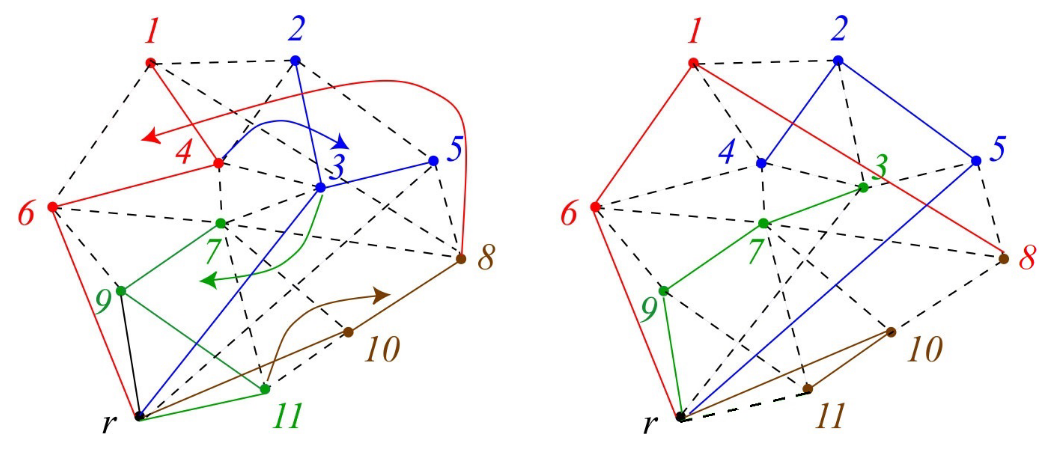
\includegraphics[width=0.9\columnwidth]{img/CMSTP1}
\end{center}
Consider the composite move $(4, {\color{blue} 3}), (3, {\color{green} 11}), (11, {\color{brown} 8}), (8, {\color{red} 4})$:
\begin{itemize}
	\item $4$ moves into the blue branch to replace $3$
	\item $3$ moves into the green branch to replace $11$
	\item $11$ moves into the brown branch to replace $8$
	\item $8$ moves into the red branch to replace $4$
\end{itemize}

The cost variation for subtree $S_j$ yields the cost of arc $c_{ij}$.\\

The weight of branch $S_j$ varies by $w_i - w_j$: if unfeasible, forbid the arc. The feasibility is determined by the single transfer, if the new cost is still feasible the transfer is feasible.\\

The total cost is the sum of all variation due to the transfers made.\\

If you visit two elements in a single component it is not guaranteed that the feasibility depends only on the single transfer.\\

\newpage

\paragraph{Search for the minimum cost circuit:} The problem is actually $\mathcal{NP}$-hard, but
\begin{itemize}
	\item The constraint of visiting only once each component allows a rather efficient \textbf{dynamic programming algorithm} that grows partial paths (if the components are $r$, the circuit has at most $r$ arcs).\\
	
	\item All \textbf{partial paths of cost} $\geq 0$ \textbf{can be neglected} because
	\begin{itemize}
		\item the total variation of the objective sums the effect of the single moves
		$$ \delta f_{o_1, \, ... \, , o_k} (x) = \sum_{\ell = 1}^k \delta f_{o_{\ell}} (x) $$
		
		\item every \textbf{sequence} of numbers \textbf{with negative sum} admits a cyclic permutation \textbf{whose partial sums are all negative}. e.g., $(+1, −2, +4, −10, +2)$ admits $(−10, +2, +1, −2, +4)$ (if the total is negative I can start with a big negative and stay in the negative all the way)
		
		\item therefore, \textbf{there is a cyclic permutation of the moves} $o_1, \, ... \, , o_k$
		$$ \delta f_{o_1, \, ... \, , o_k} (x) < 0 \implies \exists h : \, \delta f_{o_{(h+1) \mod k}, \, ... \, , o_{(h+\ell) \mod k}} (x) < 0 \text{ for } \ell = 1, \, ... \, , k $$
		that is, \textbf{improving at each step}.\\
	\end{itemize}
\end{itemize}

Moreover,
\begin{itemize}
	\item There are \textbf{heuristic polynomial algorithms} for the problem.\\
	
	\item There are \textbf{polynomial algorithms to solve relaxations} of the problem that neglect the constraint on the components, finding
	\begin{itemize}
		\item a nonminimum negative circuit (Floyd-Warshall), if any exists
		
		\item a circuit of minimum average cost (total cost divided by number of arcs)
	\end{itemize}
	If the cost of such relaxed solutions is
	\begin{itemize}
		\item positive, then no negative circuit exists
		
		\item negative, then the relaxed solution can be
		\begin{itemize}
			\item optimal (if luckily they are feasible)
			\item a starting point to generate a feasible heuristic solution
		\end{itemize}
	\end{itemize}
\end{itemize}

\newpage

\paragraph{Noncyclic exchange chains:} It is also possible to create noncyclic transfer chains, so that the cardinality of the components can vary.\\

It is enough to add to the improvement graph
\begin{itemize}
	\item A \textbf{source node} (fake, doesn't represent any node of the problem).\\
	
	\item A \textbf{node} for \textbf{each component} (a fake node for each component in the solution, for example each subtree).\\
	
	\item \textbf{Arcs} from the \textbf{source node} to the \textbf{nodes associated to the elements}.\\
	
	\item \textbf{Arcs} from the \textbf{nodes associated to the elements} to the \textbf{nodes associated to the components}.\\
\end{itemize}

Then, find the minimum cost path that
\begin{itemize}
	\item \textbf{starts} from the \textbf{source node}
	
	\item \textbf{ends} in a \textbf{component node}
	
	\item \textbf{visits at most one node for each component}
\end{itemize}

These paths correspond to \textbf{open transfer chains} in which
\begin{itemize}
	\item a component loses an element
	
	\item zero or more components lose an element and acquire another one
	
	\item a component acquires an element
\end{itemize}

You just get an element from a source node, swap $n$ elements among components, end in a component which does not lose an element.\\

\newpage

Example: the CMSTP
\begin{center}
	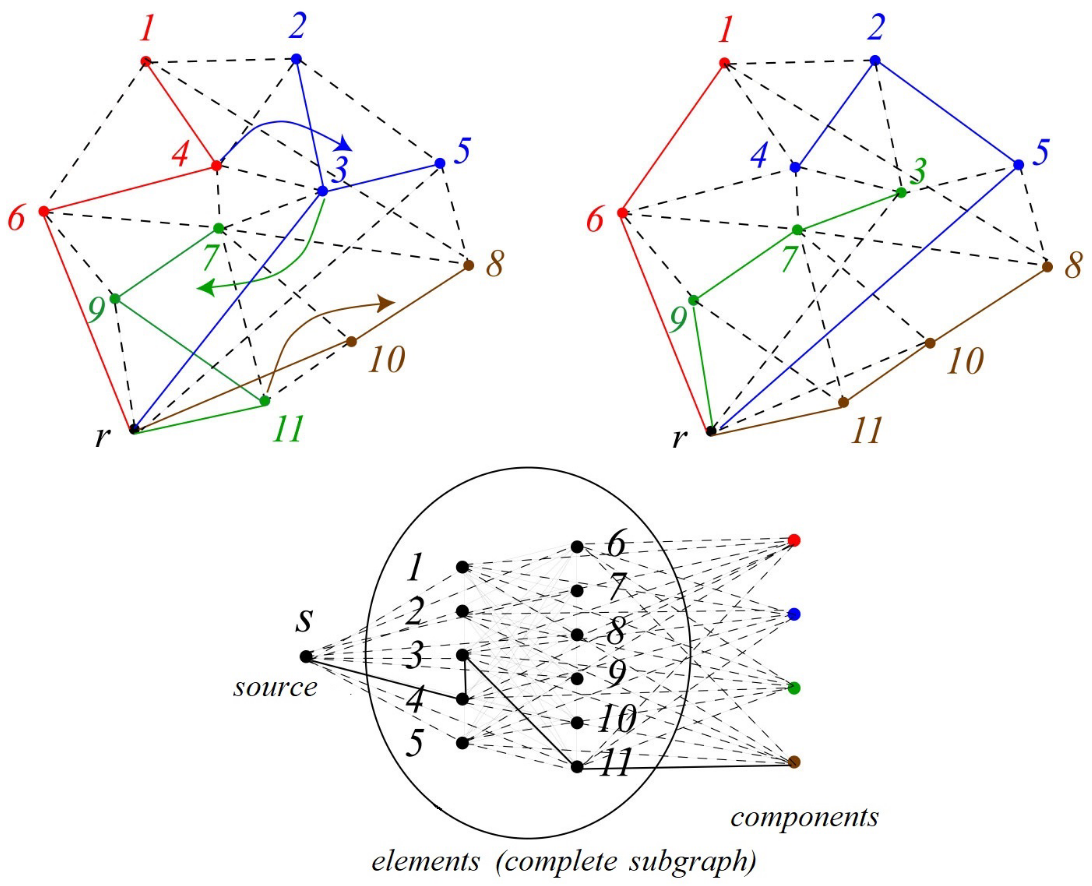
\includegraphics[width=0.9\columnwidth]{img/CMSTP2}
\end{center}
Noncyclic exchange $(s, {\color{red} 4}), (4, {\color{blue} 3}), (3, {\color{green} 11}), (11, {\color{brown} S_4})$.\\

4 goes to $s$ (it just means that we remove it), then we swap 4 and 3, and so on until in the green subtree we swap 11, which goes to brown, with $S_4$ (another fake element).\\

It's just a notation to denote empty first and last swaps.\\

\newpage

\subsection{Order-first split-second}

The \textbf{Order-first split-second} method for \textbf{partition problems}
\begin{itemize}
	\item \textbf{Builds} a \textbf{starting permutation of the elements} to be partitioned.\\
	
	\item \textbf{Partitions the elements into components in an optimum way} under the additional constraint that \textbf{elements} of the \textbf{same component} be \textbf{consecutive in the starting permutation}.\\
\end{itemize}

Of course, the solution depends on the starting permutation: it is reasonable to repeat the resolution for different permutations creating a two-level method
\begin{enumerate}
	\item the upper level selects a permutation
	
	\item the lower level computes the optimal partition for the permutation
\end{enumerate}

Problem: different permutations yield the same solution (the permutations are more numerous than the solutions).\\


\paragraph{The auxiliary graph:} Once again, we exploit an auxiliary graph. \\
Given the permutation $(s1, \, ... \, , s_n)$ of the elements
\begin{itemize}
	\item each \textbf{node} $v_i$ \textbf{corresponds to an element} $s_i$ plus a fictitious node $v_0$
	
	\item each \textbf{arc} $(v_i , v_j )$ with $i < j$ \textbf{corresponds to a potential component} $S_{\ell}$ that assigns to the same subset the elements $(s_{i+1}, \, ... \, , s_j)$
	\begin{itemize}
		\item from $s_i$ excluded
		\item to $s_j$ included
	\end{itemize}
	
	\item the \textbf{cost} $c_{v_i ,v_j}$ corresponds to the \textbf{cost of the component} $f (S_{\ell})$
	
	\item the \textbf{arc does not exist} if the \textbf{component is unfeasible}
\end{itemize}

Consequently
\begin{itemize}
	\item each path from $v_0$ to $v_n$ represents a solution (partition of elements)
	
	\item the cost of the path coincides with the cost of the partition
	
	\item the graph is \textbf{acyclic}: \textbf{finding the optimum path costs} $O (m)$ where $m \le n (n − 1) /2$ is the number of arcs
\end{itemize}

\newpage

\paragraph{Example:} the VRP. Given an instance of VRP with 5 nodes and capacity $W = 10$
\begin{center}
	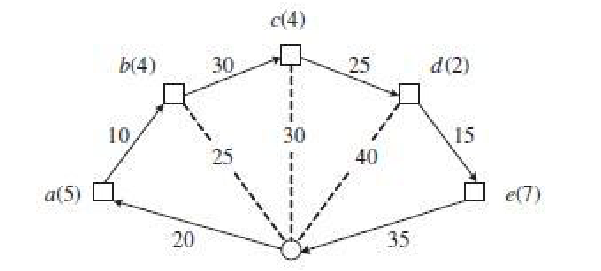
\includegraphics[width=0.6\columnwidth]{img/VRP2}
\end{center}
the arcs corresponding to unfeasible paths (weight $> W$) do not exist, the costs of the arcs are the costs of the TSP solutions for $\{d, v_{i+1}, \, ... \, , v_j \}$
\begin{center}
	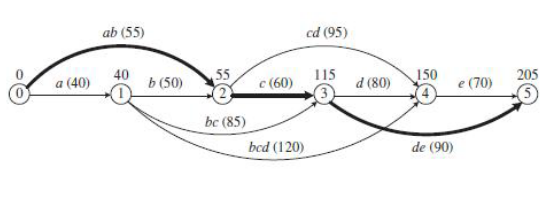
\includegraphics[width=0.6\columnwidth]{img/VRP3}
\end{center}
The optimal path corresponds to three circuits: $(d, v1, v2, d), (d, v3, d)$ and $(d, v4, v5, d)$
\begin{center}
	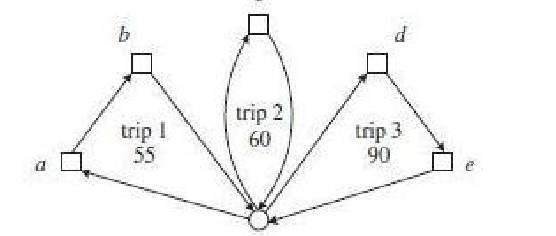
\includegraphics[width=0.6\columnwidth]{img/VRP4}
\end{center}

\newpage

\subsection{Variable Depth Search (VDS)}

In the VDS a \textbf{composite move} is a \textbf{sequence of elementary moves}
\begin{itemize}
	\item Consider each solution $x'$ in the basic neighborhood $N_{\mathcal{O}_1} (x)$.\\
	
	\item From it, make a sequence of moves \textbf{optimizing each elementary step}, but \textbf{allowing worsening moves} and \textbf{forbidding backward moves}.\\
	
	\item \textbf{Terminate} when the \textbf{current solution} $y$ becomes \textbf{worse than} $x'$ or \textbf{all moves are forbidden} (the length $k$ of the sequence is variable).\\
	
	\item \textbf{Teturn} the \textbf{best solution} $y^\ast$ \textbf{found} along the sequence.\\
\end{itemize}

\paragraph{Scheme of the VDS:} Given $x^{(t)}$, for each $x' \in N (x^{(t)})$, instead of evaluating only $f (x')$
\begin{enumerate}
	\item Find a promising solution $\tilde{y}$ in a neighborhood $\hat{N} (x') \subseteq N (x')$.\\
	
	\item As long as $\tilde{y}$ improves $x^{(t)}$, replace $x'$ with $\tilde{y}$ and go to $1$.\\
	
	\item Return the best solution $y^\ast$ found during the whole process.\\
\end{enumerate}

\newpage

\begin{center}
	For each $x' \in N (x)$
\end{center}

\begin{algorithm}
	\caption{Steepest Descent}
	\begin{algorithmic}
		\STATE Compute $f(x')$
	\end{algorithmic}
\end{algorithm}

\begin{algorithm}
	\caption{Variable Depth Search}
	\begin{algorithmic}
		\STATE $y := x'$; $y^\ast := x'$; Stop $:= false$;
		\WHILE{Stop $=false$}
		\STATE $\tilde{y} := \arg \min_{y' \in \hat{N}(y)} f(y')$
		\IF{$f (\tilde{y} ) \geq f (x')$}
		\STATE Stop $:= true$
		\ELSE
		\STATE $y := \tilde{y}$
		\ENDIF
		\IF{$f (\tilde{y} ) < f (y^\ast)$}
		\STATE $y^\ast := \tilde{y}$
		\ENDIF
		\ENDWHILE
		\RETURN $f (y^\ast)$;
	\end{algorithmic}
\end{algorithm}
It is a sort of roll-out mechanism for exchange algorithms.\\

Instead of just computing the value of the function in $x'$, you try to "launch" a local search heuristic; starting from $x'$ you repeatedly explore a neighborhood of the current solution $\tilde{y}$, as long as you don't satisfy a termination condition, keeping track of the best solution found all along.\\

You get a candidate solution and then you explore, starting from that solution, a (much) smaller neighborhood (to have a fast exploration) and repeat this cycle until a termination condition holds, i.e. when the new solution is worse than the original one.\\

By accepting worsening moves (with a bound in the original solution) it allows to go further in the search space than a simple steepest descent.\\

\newpage

\paragraph{Differences to steepest descent:} With respect to steepest descent exploration
\begin{itemize}
	\item VDS \textbf{finds a local optimum for each solution of the neighborhood} performing a sort of one-step look-ahead.\\
	
	\item VDS \textbf{admits worsenings along the sequence} of elementary moves (but never with respect to the starting solution).\\
	
	\item VDS \textbf{makes moves that increase the distance from the starting point} to avoid cyclic behaviors (gradually restricting the neighborhood).\\
\end{itemize}

In order to limit the computational effort
\begin{itemize}
	\item the \textbf{elementary moves} use a \textbf{reduced neighborhood} $\hat{N} \subseteq N$
	
	\item $\hat{N}$ (elementary step) is \textbf{explored} with the \textbf{first-best strategy} (as soon as you find an improvement you take it)
	
	\item $N$ (basic neighborhood) is \textbf{explored} with the \textbf{first-best strategy}
\end{itemize}

Instead of just computing the objective function you're trying to "have a look" far away.\\

\newpage

\subsubsection{Lin-Kernighan's algorithm for the symmetric TSP}
Still the best performing algorithm for the TSP (a variation of it).\\

Neighborhood $N_{\mathcal{R}_k} (x)$ includes the solutions obtained
\begin{itemize}
	\item deleting $k$ arcs of $x$
	
	\item adding other $k$ arcs that recreate a Hamiltonian circuit
	
	\item possibly inverting parts of the circuit (leaving the cost unchanged)
\end{itemize}

Lin-Kernighan's algorithm is a VDS with \textbf{sequences of 2-opt exchanges}: a $k$-opt exchange is equivalent to a sequence of $(k - 1)$ 2-opt exchanges, where each deletes one of the two arcs added by the previous exchange.\\

Then for each solution $x' \in N_{\mathcal{R}_2} (x)$ obtained by exchange $(i, j)$
\begin{itemize}
	\item evaluate the 2-opt exchanges that delete the added arc $(s_i , s_{j+1})$ and each arc of $x \cap x'$ to find the best exchange $(i', j')$
	
	\item if this improves upon $x$, perform exchange $(i', j')$, obtaining $x''$
	
	\item evaluate the exchanges that delete $(s_{i'}, s_{j'+1})$ and each arc of $x \cap x''$ ...
	
	\item ...
	
	\item if the best solution among $x', x'', \, ...$ is better than $x$, accept it
\end{itemize}

It essentially does a 2-opt exchange among 2 arcs and then deletes one (fixed) and takes time $O(n)$ to search the best possible exchange across all other nodes in the solution. Reverse the path among nodes when needed. Example not provided, too long (L14 slides).\\

The arc to be removed is never the one chosen after the search, always the other one, it would be a backward move otherwise.\\

\newpage

\paragraph{Implementation details:}
\begin{itemize}
	\item \textbf{Each step deletes an arc of the starting solution} to avoid going back and one of the arcs added in the previous step to reduce complexity.\\
	
	\item This imposes an \textbf{upper bound on the length of the sequence}.\\
	
	\item \textbf{Stopping the sequence as soon as the solution is no longer better than the starting solution does not impair the result}
	\begin{itemize}
		\item the total variation of the objective sums the effect of the single moves
		$$ \delta f_{o_1, \, ... \, , o_k} (x) = \sum_{\ell = 1}^k \delta f_{o_{\ell}} (x) $$
		
		\item every sequence of numbers with negative sum admits a cyclic permutation whose partial sums are all negative
		
		\item therefore, there is a cyclic permutation of the moves $o_1, \, ... \, , o_k$ that is, improving at each step (these last two points have already been discussed)
	\end{itemize}
\end{itemize}

\newpage

\subsection{Iterated greedy methods (destroy-and-repair)}

Every \textbf{exchange} can be seen as a \textbf{combination of addition and deletion}
$$ x' = x \cup A \setminus D $$
with $A = x' \setminus x$ and $D = x \setminus x'$.\\

However
\begin{itemize}
	\item single swaps $x' = x \cup \{j\} \setminus \{i\}$ \textbf{can give bad or unfeasible results}
	
	\item \textbf{larger neighborhoods} can be \textbf{inefficient}
	
	\item in many problems \textbf{the right cardinalities of} $A$ \textbf{and} $D$ \textbf{are unknown}, because the solutions have nonuniform cardinality (e.g., KP, SCP. . . )
\end{itemize}

A possible idea is to
\begin{enumerate}
	\item \textbf{delete from} $x$ a \textbf{subset} $D \subset x$ of \textbf{cardinality} $\leq k$ (destroy heuristic)
	\item \textbf{complete it with a constructive heuristic} (repair heuristic)
\end{enumerate}

\textbf{or}, of course, \textbf{the opposite}
\begin{enumerate}
	\item add to $x$ a set $A \subset B \setminus x$ of cardinality $\leq k$
	\item reduce it with a destructive heuristic4
\end{enumerate}

\paragraph{Selection of $A$ and $D$:} Most of the time both subsets are chosen heuristically, not exhaustively
\begin{itemize}
	\item tuning their size $|A|$ and $|D|$ with some parameter
	
	\item selecting promising elements based on their cost/value
	
	\item applying the first-best strategy (immediately accept any improving solution)
\end{itemize}

Usually both subsets are chosen in a randomized way (metaheuristics then). \\

% End of L15, L16 is lab, L17 ahead

\newpage

\subsection{Overcoming local optima}
The steepest descent exchange heuristics only provide local optima.\\

In order to \textbf{improve}, one can
\begin{itemize}
	\item \textbf{repeat} the search (How to avoid following the same path?)
	\item \textbf{extend} the search (How to avoid falling in the same optimum? If I start in a neighborhood of my local optimum chances are I'll fall back into it)
\end{itemize}

In the constructive algorithms only repetition was possible.\\

The constructive metaheuristics exploit \textbf{randomization} and \textbf{memory} to operate on $\Delta_A^+ (x)$ and $\varphi_A (i, x)$.\\

The \textbf{exchange metaheuristics} exploit them to operate on
\begin{itemize}
	\item the \textbf{starting solution} $x^{(0)}$ (multi-start, ILS, VNS)
	\item the \textbf{neighborhood} $N (x)$ (VND)
	\item the \textbf{selection criteria} $\varphi (x, A, D)$ (DLS/GLS)
	\item the \textbf{selection rule} $\arg \min$ (SA, TS)
\end{itemize}

\newpage

\subsubsection{Termination condition} 

A search that repeats or extends beyond a local optimum can ideally be infinite. If you prolong the search, when does it end? \\

In pratice, one uses \textbf{termination conditions} that can be "\textbf{absolute}"
\begin{enumerate}
	\item A given \textbf{total number of explorations of the neighborhood} or a given \textbf{total number of repetitions of the local search}.\\
	
	\item A given \textbf{total execution time}.\\
	
	\item A given \textbf{value of the objective}.\\
\end{enumerate}

or "\textbf{relative}" to the \textbf{profile of} $f^\ast$
\begin{enumerate}
	\item A given \textbf{number of explorations} of the neighborhood or repetitions \textbf{after the last improvement of} $f^\ast$.\\
	
	\item A given \textbf{execution time after the last improvement}.\\
	
	\item A given \textbf{minimum value of the ratio between improvement} of the objective and \textbf{number of explorations/repetitions} or \textbf{execution time} (e.g.: $f^\ast$ improves less than $1\%$ in the last $1000$ explorations).\\
\end{enumerate}

\textbf{Fair comparisons} require \textbf{absolute conditions} (give both the same time/number of exploration).\\

\newpage

\subsection{Modify the starting solution}

It is possible to create \textbf{different starting solutions}
\begin{itemize}
	\item Generating them at \textbf{random}
	\begin{itemize}
		\item with uniform probability
		\item with biased distributions (based on the data, possibly on memory)
	\end{itemize}
	\nn
	
	\item Applying different \textbf{constructive algorithms}
	\begin{itemize}
		\item heuristics
		\item metaheuristics (with randomization and/or memory)
	\end{itemize}
	\nn
	
	\item Applying the \textbf{exchange algorithm to modify the solutions visited} (therefore with memory, and usually also randomization)
\end{itemize}

\newpage

\subsubsection{Random generation}

The \textbf{advantages} of random generation are
\begin{itemize}
	\item Conceptual \textbf{simplicity}.\\
	
	\item \textbf{Quickness} for the problems in which it is easy to guarantee feasibility.\\
	
	\item \textbf{Control} on the \textbf{probability distribution} in $X$ based on
	\begin{itemize}
		\item element cost (e.g., favor the cheapest elements)
		
		\item element frequency during the past search, to favor the most frequent elements (intensification) or the less frequent ones (diversification). This combines randomization and memory
	\end{itemize}
	\nn
	
	\item \textbf{Asymptotic convergence to the optimum} (in infinite time).\\
\end{itemize}


The \textbf{disadvantages} of random generation are
\begin{itemize}
	\item \textbf{Scarce quality} of the \textbf{starting solutions} (not the final ones).\\
	
	\item \textbf{Long times} before \textbf{reaching the local optimum}. This depends on the complexity of the exchange algorithm.\\
	
	\item \textbf{Inefficiency} when deciding feasibility is $\mathcal{NP}$-complete.\\
\end{itemize}

\newpage

\subsubsection{Constructive procedures}

Multi-start methods are the classical approach
\begin{itemize}
	\item design \textbf{several constructive heuristics}
	\item \textbf{each} constructive heuristic \textbf{generates a starting solution}
	\item \textbf{each starting solution} is \textbf{improved} by the \textbf{exchange heuristic}
\end{itemize}

\nn

The disadvantages are
\begin{enumerate}
	\item \textbf{scarce control}: the generated solutions tend to be similar
	
	\item \textbf{impossibility to proceed indefinitely}: the number of repetitions is fixed
	
	\item \textbf{high design effort}: several different algorithms must be designed
	
	\item \textbf{no guarantee of convergence}, not even in infinite time
\end{enumerate}

Consequently, constructive metaheuristics are preferred nowadays. The initial step is given by a constructive metaheuristic. \\

GRASP and Ant System include by definition an exchange procedure.\\

What's the difference between a metaheuristic with a randomized/memory based constructive phase and an exchange heuristic with initialized by a randomized process? There's little difference.\\

\newpage

\subsubsection{Influence of the starting solution}
The starting solution obviously has influence on the algorithm's performance, so how do we determine if we can choose a random generation or if we need a good constructive heuristic?\\

If the \textbf{exchange heuristic} is
\begin{itemize}
	\item \textbf{Good}, the starting solution has a \textbf{short-lived influence}: a random or heuristic generation of $x^{(0)}$ are very similar.\\
	
	\item \textbf{Bad}, the starting solution has a \textbf{long-lived influence}: a good heuristic to generate $x^{(0)}$ is useful.\\
\end{itemize}
If the heuristic is not good, it might be a good idea to spend some time generating the starting solution, while if the exchange phase is very good the starting solution doesn't matter as much.\\

\begin{center}
	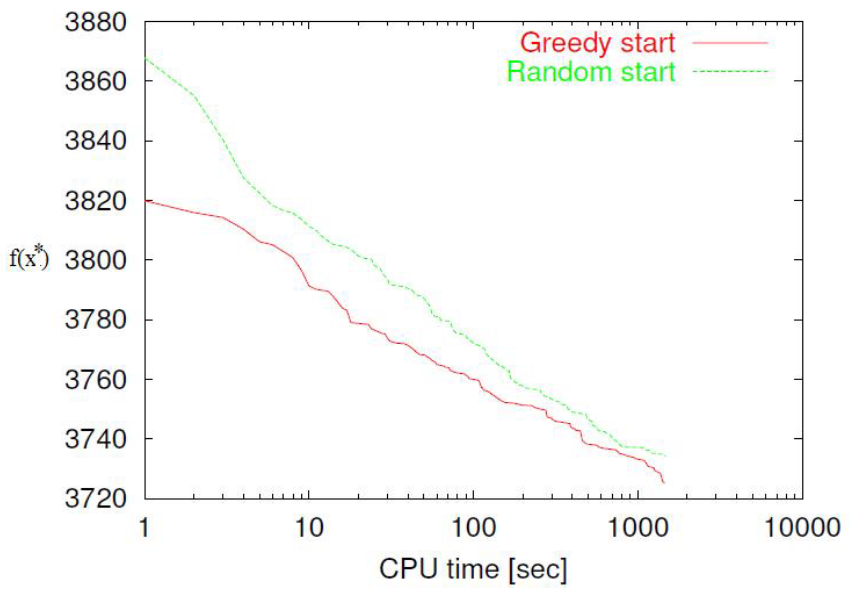
\includegraphics[width=0.8\columnwidth]{img/influence1}
\end{center}
\textit{This exchange heuristic is not very good, there's still a perceivable (albeit small) difference at the end, after a significant amount of time (note the logarithmic scale).}

\newpage

\subsubsection{Exploiting the previous solutions}
The idea is to \textbf{exploit the information on previously visited solutions}
\begin{itemize}
	\item save \textbf{reference solutions}, such as the best local optimum found so far and possibly other local optima
	
	\item \textbf{generate the new starting solution modifying the reference ones}
\end{itemize}

During the exchange heuristic you save some solutions that are "interesting" (the best, possibly others, usually good-quality solutions) and generate some other starting solutions based on these.\\ 

The advantages of this approach are
\begin{itemize}
	\item \textbf{control}: the modification can be reduced or increased \textit{ad libitum}. You can intensify or diversify the search at will (in respect to the starting point)
	
	\item \textbf{good quality}: the starting solution is very good (you start from a good-quality solution)
	
	\item \textbf{conceptual simplicity}: just design a modification, no need to invent much new stuff
	
	\item \textbf{implementation simplicity}: the modification can be performed with the operations defining the neighborhood
	
	\item \textbf{asymptotic convergence to the optimum} under suitable conditions
\end{itemize}

\newpage

\subsection{Iterated Local Search (ILS)}

The Iterated Local Search (ILS), proposed by Louren¸co, Martin and St\"utzle (2003) requires
\begin{itemize}
	\item a \textbf{steepest descent} exchange heuristic to \textbf{produce local optima}
	
	\item a \textbf{perturbation procedure} to \textbf{generate the starting solutions}
	
	\item an \textbf{acceptance condition} to decide whether to \textbf{change the reference solution} $x$
	
	\item a \textbf{termination condition}
\end{itemize}

\begin{algorithm}
	\caption{Algorithm $IteratedLocalSearch(I , x^{(0)})$}
	\begin{algorithmic}
		\STATE $x := SteepestDescent(x^{(0)})$
		\STATE $x^\ast := x$
		\FOR{$l := 1$ to $\ell$}
		\STATE $x' := Perturbate(x)$
		\STATE $x' := SteepestDescent(x')$
		\IF{$Accept(x', x^\ast)$} 
		\STATE $x := x'$
		\ENDIF
		\IF{$f (x') < f (x^\ast)$}
		\STATE $x^\ast := x'$
		\ENDIF
		\ENDFOR
		\RETURN $(x^\ast, f (x^\ast))$
	\end{algorithmic}
\end{algorithm}

It iteratively applies local search by generating new starting solutions every time, so you need an exchange heuristic on which to base this on.\\

The perturbation procedure is used to generate new starting solutions from the reference.\\

The acceptance condition is needed to decide if the local optimum found can be accepted as the new reference (otherwise the old one is kept and "perturbed" for a new starting solution).\\

In the end it returns the best solution found.

\newpage

The idea is that
\begin{itemize}
	\item The \textbf{exchange heuristic quickly explores an attraction basin}, terminating into a local optimum.
	
	\item The \textbf{perturbation procedure moves to another attraction basin}.
	
	\item The \textbf{acceptance condition evaluates if the new local optimum is a promising starting point} for the following perturbation.
\end{itemize}

\begin{center}
	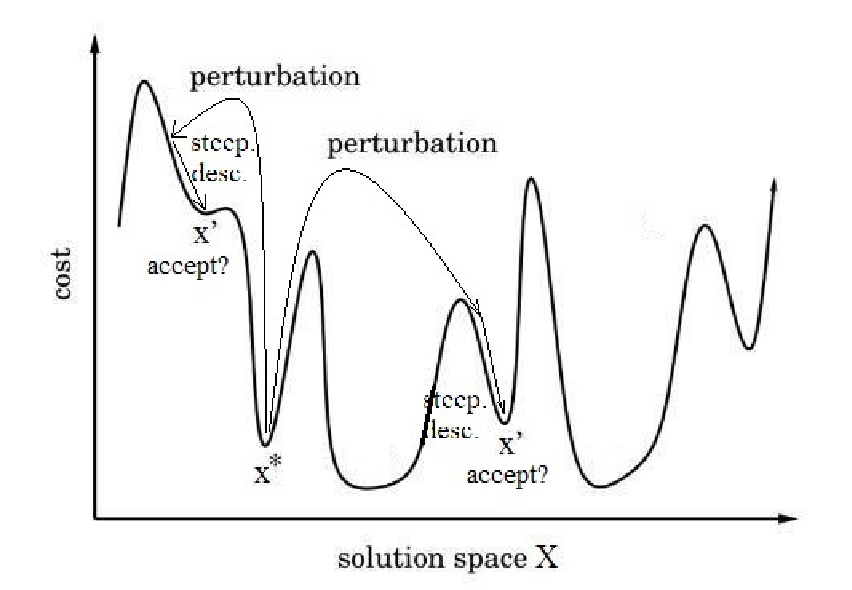
\includegraphics[width=0.7\columnwidth]{img/ILS1}
\end{center}

\vfill

\paragraph{Example:} A classical application of ILS to the TSP uses
\begin{itemize}
	\item exchange heuristic: steepest descent with neighborhood $N_{\mathcal{R}_2}$ (remove 2 edges)
	
	\item perturbation procedure: a double-bridge move that is particular kind of 4-exchange
	\begin{center}
		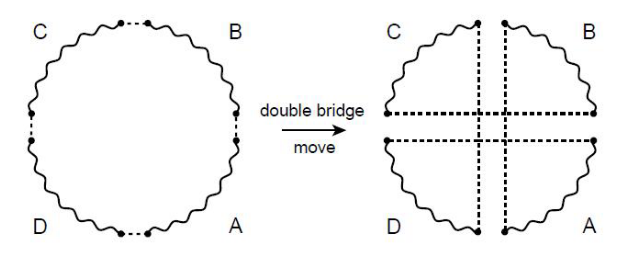
\includegraphics[width=0.6\columnwidth]{img/TSP5}
	\end{center}
	
	\item acceptance condition: the best known solution improves 
	$$f (x') < f (x^\ast)$$
	The reference solution is the best known one ($x = x^\ast$)
\end{itemize}

\newpage

\subsubsection{Perturbation procedure}

Let $\mathcal{O}$ be the operation set that defines neighborhood $N_{\mathcal{O}}$.\\

The \textbf{perturbation procedure} performs a \textbf{random operation} $o$
\begin{itemize}
	\item with $o \in \mathcal{O}' \not \subseteq \mathcal{O}$, to avoid the exchange heuristic driving solution $x'$ back to the starting local optimum $x$ (you need a new starting point, go far enough to get one)
\end{itemize}

Two typical definitions of $\mathcal{O}'$ are
\begin{itemize}
	\item \textbf{sequences of} $k > 1$ \textbf{operations of} $\mathcal{O}$ (generating a random sequence is cheap)
	
	\item \textbf{conceptually different operations} (e.g., vertex exchanges instead of edge exchanges)
\end{itemize}

The main difficulty of ILS is in tuning the perturbation: if it is
\begin{itemize}
	\item \textbf{Too strong}, it turns the search into a \textbf{random restart} (if you go way too far it's just a new random start).\\
	
	\item \textbf{Too weak}, it guides the search back to the \textbf{starting local optimum} (you are too close to the previous one)
	\begin{itemize}
		\item wasting time
		\item possibly losing the asymptotic convergence
	\end{itemize}
	\nn
\end{itemize}

Ideally one would like to \textbf{enter any basin} and \textbf{get out of any basin} (and the perturbation must be tuned according to the specific basin).\\

\newpage

\subsubsection{Acceptance condition}
The acceptance condition \textbf{balances intensification and diversification}
\begin{itemize}
	\item Accepting \textbf{only improving solutions} favors \textbf{intensification}
	$$Accept(x', x^\ast) := (f (x') < f (x^\ast))$$
	The reference solution is always the best found: $x = x^\ast$.\\
	
	\item Accepting \textbf{any solution} favors \textbf{diversification}
	$$ Accept(x', x^\ast) := true $$
	The reference solution is always the last optimum found: $x = x'$.\\
\end{itemize}

\textbf{Intermediate strategies} can be defined \textbf{based on} $\delta f = f (x') - f (x^\ast)$ the difference in the objective function
\begin{itemize}
	\item if $\delta f < 0$, \textbf{always accept} $x'$
	
	\item if $\delta f \geq 0$, \textbf{accept} $x'$ \textbf{with probability} $\pi (\delta f)$, where $\pi (\cdot)$ is a nonincreasing function
\end{itemize}

The most \textbf{typical cases} are:
\begin{itemize}
	\item \textbf{constant probability}: $\pi (\delta f ) = \overline{\pi} \in (0; 1)$ for each $\delta f \geq 0$
	
	\item \textbf{monotonically decreasing probability} with $\pi (0) = 1$ and $\lim_{\delta f \rightarrow + \infty} \pi (\delta) = 0$; the probability decreases proportionally to the worsening of the solution
\end{itemize}

\begin{center}
	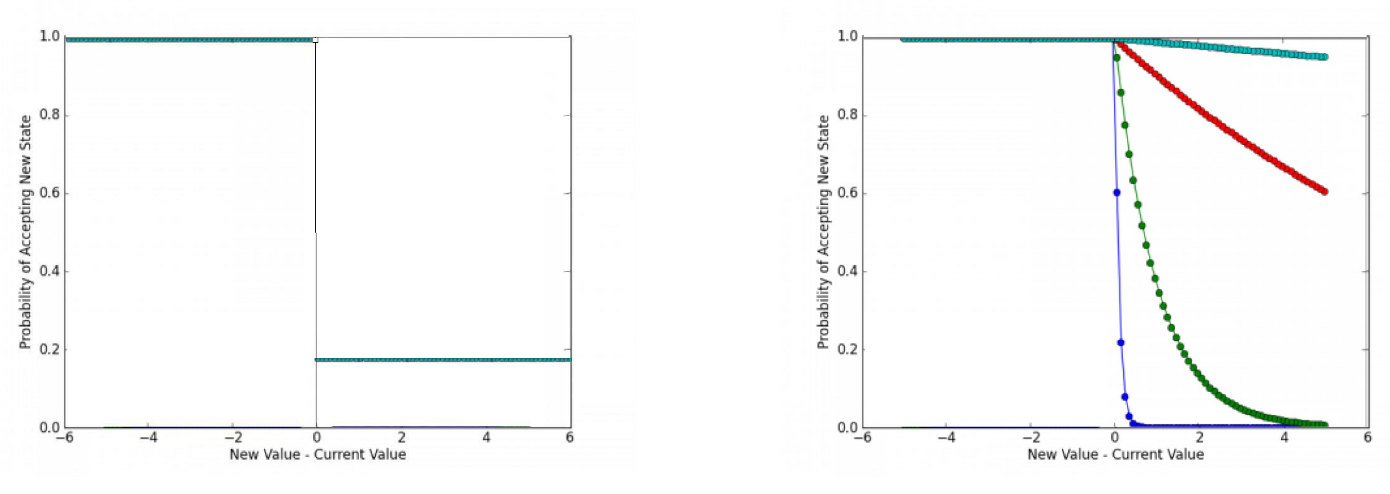
\includegraphics[width=\columnwidth]{img/accept1}
\end{center}

\textbf{Memory} can also be used, \textbf{accepting} $x'$ \textbf{more easily if many iterations have elapsed since the last improvement of} $x^\ast$.\\

\newpage

\subsection{Variable Neighborhood Search (VNS)}

A method very similar to ILS is the Variable Neighborhood Search proposed by Hansen and Mladenovi\'c (1997).\\

The \textbf{main differences} between ILS and VNS are the \textbf{use of}
\begin{itemize}
	\item The \textbf{strict acceptance condition}: $f (x') < f (x^\ast)$ (only intensifies, simpler).\\
	
	\item An \textbf{adaptive perturbation mechanism} instead of the fixed one (more complicated than ILS).\\
\end{itemize}

VNS often introduces also neighborhood modifications (later on this).\\

The \textbf{perturbation mechanism} is based on a \textbf{hierarchy of neighborhoods}, that is a \textbf{family of neighborhoods with an increasing parametric size} $s$
$$ N_1 \subset N_2 \subset \, ... \, \subset N_s \subset \, ... \, N_{s_{max}} $$


Typically the parameterized neighborhoods used are
\begin{itemize}
	\item $N_{\mathcal{H}_s}$, based on the Hamming distance between subsets
	
	\item $N_{\mathcal{O}_s}$, based on the sequences of operations from a basic set $\mathcal{O}$
\end{itemize}

and $x^{(0)}$ is extracted randomly from a neighborhood of the hierarchy.\\

\newpage

\begin{algorithm}
	\caption{Algorithm $VariableNeighbourhoodSearch(I , x^{(0)}, s_{min}, s_{max}, \delta s)$}
	\begin{algorithmic}
		\STATE $x := SteepestDescent(x^{(0)})$ 
		\STATE $x^\ast := x$
		\STATE $s := s_{min}$
		\FOR{$l := 1$ to $\ell$}
		\STATE $x' := Shaking(x^\ast, s)$
		\STATE $x' := SteepestDescent(x')$
		\IF{$f (x') < f (x^\ast)$}
		\STATE $x^\ast := x'$
		\STATE $s := s_{min}$
		\ELSE 
		\STATE $s := s + \delta s$
		\ENDIF
		\IF{$s > s_{max}$}
		\STATE $s := s_{min}$
		\ENDIF
		\ENDFOR
		\RETURN $(x^\ast, f (x^\ast))$
	\end{algorithmic}
\end{algorithm}

\begin{itemize}
	\item the \textbf{reference solution} $x'$ is \textbf{always the best known} solution $x^\ast$
	
	\item the \textbf{starting solution} is obtained extracting it at \textbf{random from the current neighborhood of the reference solution} $N_s (x^\ast)$
	
	\item the \textbf{exchange heuristic} produces a \textbf{local optimum} with respect to the \textbf{basic neighborhood} $N$
	
	\item if the \textbf{best known solution improves}, the \textbf{current neighborhood becomes} $N_{s_{min}}$
	
	\item \textbf{otherwise, move to a larger neighborhood} $N_{s+\delta s}$, never exceeding $N_{s_{max}}$
\end{itemize}

\newpage

\subsubsection{Adaptive perturbation mechanism}
It is called \textbf{variable neighborhood} because the \textbf{neighborhood used to extract} $x^{(0)}$ \textbf{varies} based on the results of the exchange heuristic
\begin{itemize}
	\item \textbf{if a better solution is found}, use the \textbf{smallest neighborhood}, to generate a starting solution very close to $x^\ast$ (intensification)
	
	\item \textbf{if a worse solution is found}, use a \textbf{slightly larger neighborhood}, to generate a starting solution slightly farther from $x^\ast$ (diversification)
\end{itemize}

If you find a better solution you accept it and set $s$ to the minimum possible value, the new starting solution is close to the current one (you get closer, perturb only a little).\\
If you find a worse solution you perturbed too little, you need to increase $s$ and perturb more (starting solution that is farther away from the current one).\\


The method has \textbf{three parameters}
\begin{enumerate}
	\item $s_{min}$ identifies the \textbf{smallest neighborhood to generate new solutions}
	
	\item $s_{max}$ identifies the \textbf{largest neighborhood to generate new solutions}
	
	\item $\delta_s$ is the \textbf{increase of} $s$ \textbf{between two subsequent attempts} (how much does the neighborhood increase when it fails?)
\end{enumerate}

The exchange heuristic adopts a \textbf{small neighborhood to be efficient} ($N_1$, or anyway $N_s$ with $s \leq s_{min}$).\\

\newpage

\paragraph{Tuning of the shaking parameters:} The value of $s_{min}$ must be
\begin{itemize}
	\item \textbf{Large enough} to get \textbf{out of the current attraction basin}.\\
	
	\item \textbf{Small enough} to \textbf{avoid jumping over the adjacent attraction basins}.\\
\end{itemize}

In general, one sets $s_{min} = 1$, and increases it if experimentally profitable.\\

The value of $s_{max}$ must be
\begin{itemize}
	\item \textbf{Large enough} to \textbf{reach any useful attraction basin}.\\
	
	\item \textbf{Small enough} to \textbf{avoid reaching useless regions} of the solution space.\\
\end{itemize}
Example: the diameter of the search space for the basic neighborhood: $min (k, n - k)$ for the MDP; $n$ for the TSP and MAX-SAT, etc.\\

The value of $\delta s$ must be
\begin{itemize}
	\item \textbf{Large enough} to \textbf{reach} $s_{max}$ \textbf{in a reasonable time}.\\
	
	\item \textbf{Small enough} to \textbf{allow each reasonable value of} $s$.\\
\end{itemize}

In general, one sets $\delta s = 1$, unless $s_{max} - s_{min}$ is too large.\\

\newpage

\subsubsection{Skewed VNS}
In order to \textbf{favor diversification}, it is possible to \textbf{accept} $x'$ \textbf{when}
$$ f (x') < f (x^\ast) + \alpha d_H (x', x^\ast) $$
where
\begin{itemize}
	\item $d_H (x', x^\ast)$ is the \textbf{Hamming distance} between $x'$ and $x^\ast$
	
	\item $\alpha > 0$ is a \textbf{suitable parameter}
\end{itemize}
Accept bounded worsening solution, if they're far enough away (measured with the Hamming distance). How distant they are determines how much worse they can get.\\

This allows to \textbf{accept worsening solutions} as long as they are \textbf{far away}
\begin{itemize}
	\item $\alpha \approx 0$ tends to accept only improving solutions
	
	\item $\alpha \gg 0$ tends to accept any solution
\end{itemize}
The parameter $\alpha$ is the "worsening bound", determines how much worse the solution can get and still get accepted (if it's far enough away).\\

Of course, the random strategies seen for the ILS can also be adopted.\\

% End of L17

\newpage

\subsection{Extending the local search without worsening}

Instead of repeating the local search, \textbf{extend it beyond the local optimum}.\\

To \textbf{avoid worsening} solutions, the \textbf{selection step must be modified}
$$ \tilde{x} := \arg \min_{x' \in N(x)} f (x') $$

And two main strategies allow doing that
\begin{itemize}
	\item The \textbf{Variable Neighborhood Descent} (VND), \textbf{changes the neighborhood} $N$
	\begin{itemize}
		\item it guarantees an evolution with no cycles (the objective improves)
		\item it terminates when all neighborhoods have been exploited
	\end{itemize}
	\nn
	
	\item The \textbf{Dynamic Local Search} (DLS) \textbf{changes the objective function} $f$ ($\tilde{x}$ is better than $x$ for the new objective, possibly worse for the old)
	\begin{itemize}
		\item it can be trapped in loops (the new objective changes over time)
		\item it can proceed indefinitely
	\end{itemize}
	\nn
\end{itemize}

\newpage

\subsection{Variable Neighborhood Descent (VND)}

The Variable Neighborhood Descent of Hansen and Mladenovi\'c (1997) exploits the fact that a \textbf{solution is locally optimal for a specific neighborhood}
\begin{itemize}
	\item a \textbf{local optimum} can be \textbf{improved} using a \textbf{different neighborhood}
\end{itemize}
If you change the neighborhood, the local optimum changes.\\

Given a \textbf{family of neighborhoods} $N_1, \, ... \, , N_{s_{tot}}$
\begin{enumerate}
	\item set $s := 1$
	\item apply a \textbf{steepest descent exchange heuristic} and find a \textbf{local optimum} $\overline{x}$ \textbf{with respect to} $N_s$
	\item \textbf{flag all neighborhoods} for which $\overline{x}$ \textbf{is locally optimal and update} $s$
	\item if $\overline{x}$ is a local optimum for all $N_s$, terminate; otherwise, go back to point 2
\end{enumerate}

\begin{algorithm}
	\caption{Algorithm $VariableNeighbourhoodDescent(I , x^{(0)})$}
	\begin{algorithmic}
		\STATE $flag_s := false \; \forall k$
		\STATE $\overline{x} := x^{(0)}$ 
		\STATE $x^\ast := x^{(0)}$
		\STATE $s := 1$
		\WHILE{$\exists s : flag_s = false$}
		\STATE $\overline{x} := SteepestDescent(\overline{x}, s)$ // possibly truncated
		\STATE $flag_s := true$
		\IF{$f (\overline{x}) < f (x^\ast)$}
		\STATE $x^\ast := \overline{x}$
		\STATE $flag_{s'} := false \; \forall s' \neq s$
		\ENDIF
		\STATE $s := Update(s)$
		\ENDWHILE
		\RETURN $(x^\ast, f (x^\ast))$
	\end{algorithmic}
\end{algorithm}

\newpage

\paragraph{Anticipated termination of Steepest Descent:} Using many neighborhoods means that some might be rather \textbf{large} and \textbf{slow to explore}.\\

In order to increase the efficiency of the method one can
\begin{itemize}
	\item Adopt a \textbf{first-best strategy in the larger neighborhoods}.\\
	
	\item \textbf{Terminate the Steepest Descent before reaching a local optimum} (possibly even after a single step).\\
	
\end{itemize}
Larger neighborhoods aim to \textbf{move out of the basins of attraction of smaller ones}.\\

\nn

\paragraph{VND and VNS:} There is of course a strict relation between VND and VNS (in fact, they were proposed in the same paper).\\

The \textbf{fundamental differences} are that in the VND
\begin{itemize}
	\item At each step the \textbf{current solution is the best known one}.\\
	
	\item The \textbf{neighborhoods are explored}, instead of being used to extract random solutions; they are never huge.\\
	
	\item The \textbf{neighborhoods do not necessarily form a hierarchy}; the update of $s$ is not always an increment.\\
	
	\item When a \textbf{local optimum for each} $N_s$ \textbf{has been reached}, \textbf{terminate}; VND is deterministic and would not find anything else.\\
\end{itemize}

\newpage

\subsubsection{Neighborhood update strategies for the VND}

There are two main classes of VND methods
\begin{itemize}
	\item Methods with \textbf{heterogeneous neighborhoods}
	\begin{itemize}
		\item exploit the potential of \textbf{topologically different neighborhoods} (e.g., exchange vertices instead of edges)
	\end{itemize}
	Consequently, $s$ periodically scans the values from $1$ to $s_{tot}$ (possibly randomly permuting the sequence at each repetition).\\
	
	\item Methods with \textbf{hierarchical neighborhoods} ($N_1 \subset \, ... \, \subset N_{s_{tot}}$)
	\begin{itemize}
		\item \textbf{fully exploit} the \textbf{small and fast neighborhoods}
		\item resort to the \textbf{large and slow ones only to get out of local optima} (usually terminating Steepest Descent prematurely)
	\end{itemize}
	Consequently, the update of $s$ works as in the VNS
	\begin{itemize}
		\item when \textbf{no improvements} can be found in $N_s$, \textbf{increase} $s$
		\item when \textbf{improvements} can be found in $N_s$, \textbf{decrease} $s$ back to $1$
	\end{itemize}
\end{itemize}

\textbf{Terminate when the current solution is a local optimum for all} $N_s$
\begin{itemize}
	\item in the \textbf{heterogeneous case}, terminate when \textbf{all fail}
	\item in the \textbf{hierarchical case}, terminate when the \textbf{largest fails}
\end{itemize}

\newpage

\paragraph{Example:} This instance of CMSTP has $n = 9$ vertices, uniform weights ($w_v = 1$), capacity $W = 5$ and the reported costs (graph is complete but the missing edges have $c_e \gg 3$, so they are not drawn).

\begin{center}
	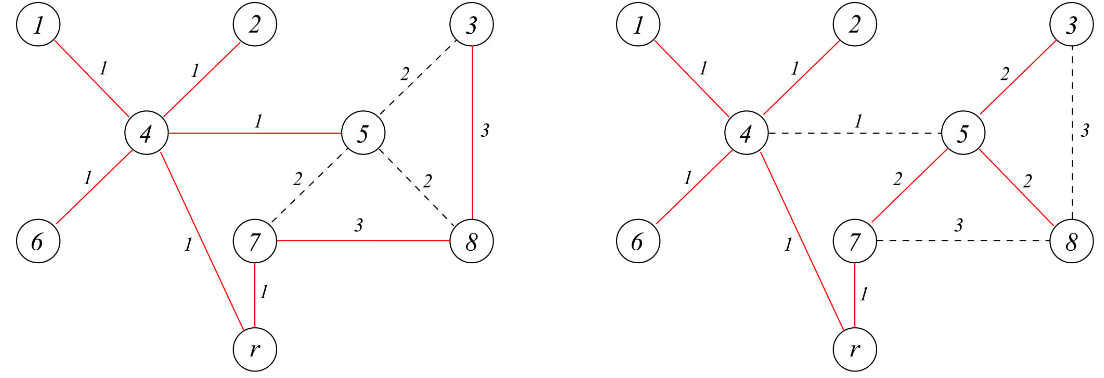
\includegraphics[width=\columnwidth]{img/CMST4}
\end{center}

Consider neighborhood $N_{\mathcal{S}_1}$ (single-edge swaps) for the first solution:
\begin{itemize}
	\item no edge in the right branch can be deleted because the left branch has zero residual capacity and a direct connection to the root would increase the cost
	
	\item deleting any edge in the left branch increases the total cost, the solution is a local optimum for $N_{\mathcal{S}_1}$
\end{itemize} 

Neighborhood $N_{\mathcal{T}_1}$ (single-vertex transfers) has an improving solution, obtained moving vertex $5$ from the left branch to the right one.\\

On the left the solution for $N_{\mathcal{S}_1}$, on the right the one for $N_{\mathcal{T}_1}$ (obviously the case of heterogeneous neighborhoods).\\

\newpage

\subsection{Dynamic Local Search (DLS)}

The Dynamic Local Search is also known as Guided Local Search.\\

Its approach is \textbf{complementary} to VND
\begin{itemize}
	\item it \textbf{keeps the starting neighborhood}
	\item it \textbf{modifies the objective function}
\end{itemize}

It is often used when the \textbf{objective is useless} because it has \textbf{wide plateaus} (e.g. in the PMSP the completion time is often the same, even after multiple movements).\\

The \textbf{basic idea} is to
\begin{itemize}
	\item Define a \textbf{penalty function} $w : X \rightarrow \mathbb{N}$ (defined on the solution, usually integer values).\\
	
	\item Build an \textbf{auxiliary function} $\tilde{f} (f (x) , w (x))$ which \textbf{combines the objective function} $f$ \textbf{with the penalty} $w$.\\
	
	\item Apply a \textbf{steepest descent exchange heuristic to optimize} $\tilde{f}$.\\
	
	\item At each iteration \textbf{update the penalty} $w$ \textbf{based on the results} (and consequently update the function $\tilde{f}$ and the landscape of the search).\\
\end{itemize}

The penalty is adaptive in order to move away from recent local optima but this introduces the risk of cycling.\\

\newpage

\begin{algorithm}
	\caption{Algorithm $DynamicLocalSearch(I , x^{(0)})$}
	\begin{algorithmic}
		\STATE $w := StartingPenalty(I )$
		\STATE $\overline{x} := x^{(0)}$
		\STATE $x^\ast := x^{(0)}$
		\WHILE{$Stop() = false$}
		\STATE $(\overline{x}, x_f) := SteepestDescent(\overline{x}, f , w )$ // possibly truncated
		\IF{$f (x_f ) < f (x^\ast)$}
		\STATE $x^\ast := x_f$
		\ENDIF
		\STATE $w := UpdatePenalty(w, \overline{x}, x^\ast)$
		\ENDWHILE
		\RETURN $(x^\ast, f (x^\ast))$
	\end{algorithmic}
\end{algorithm}
Notice that the steepest descent heuristic
\begin{itemize}
	\item \textbf{Optimizes a combination} $\tilde{f}$ \textbf{of} $f$ \textbf{and} $w$ (Steepest Descent is applied to both).\\
	
	\item \textbf{Returns two solutions}:
	\begin{enumerate}
		\item a \textbf{final solution} $\overline{x}$, locally \textbf{optimal} with \textbf{respect to} $\tilde{f}$, \textbf{to update} $w$
		\item a \textbf{solution} $x_f$, that is the \textbf{best it has found with respect to} $f$
	\end{enumerate}
\end{itemize}

\newpage

\subsubsection{Variants}

The \textbf{penalty can be applied} (for example)
\begin{itemize}
	\item \textbf{Additively} to the elements of the solution:
	$$ \tilde{f} (x) = f (x) + \sum_{i \in x} w_i $$
	The function becomes the sum of the objective with the sum of the penalties for all elements in the solution; each element is penalized, it searches for elements with low penalty.\\
	
	\item \textbf{Multiplicatively} to components of the objective $f (x) = \sum_j \phi_j (x)$:
	$$ \tilde{f} (x) = \sum_j w_j \phi_j (x) $$
	The objective function is defined in terms of components and each one is multiplied by its penalty.\\
\end{itemize}

The \textbf{penalty} can be \textbf{updated}
\begin{itemize}
	\item at \textbf{each} single \textbf{neighborhood exploration}
	
	\item when a \textbf{local optimum for} $\tilde{f}$ \textbf{is reached}
	
	\item when the \textbf{best known solution} $x^\ast$ \textbf{is unchanged for a long time}
\end{itemize}
\nn

The \textbf{penalty} can be \textbf{modified} with
\begin{itemize}
	\item \textbf{Random updates}: "noisy" perturbation of the costs.\\
	
	\item \textbf{Memory-based updates}, favoring the most frequent elements (intensification) or the less frequent ones (diversification).\\
\end{itemize}

These two are not the only ways, they are just examples, more can be defined.\\

\newpage

\paragraph{Example:} DLS for the MCP. Given an undirected graph, find a maximum cardinality clique (subset of vertices that are fully connected)
\begin{itemize}
	\item The exchange heuristic is a VND using the neighborhoods
	\begin{enumerate}
		\item $N_{\mathcal{A}_1}$ (vertex addition): the solution always improves, but the neighborhood is very small and often empty
		
		\item $N_{\mathcal{S}_1}$ (exchange of an internal vertex with an external one): the neighborhood is larger, but forms a plateau (uniform objective)
	\end{enumerate}
	\nn
	
	\item The objective provides no useful direction in either neighborhood.\\
	
	\item Associate to each vertex $i$ a penalty $w_i$ initially equal to zero.\\
	
	\item The exchange heuristic minimizes the total penalty (within the neighborhood).\\
	
	\item Update the penalty
	\begin{enumerate}
		\item when the exploration of $N_{\mathcal{S}_1}$ terminates: the penalty of the current clique vertices increases by $1$
		
		\item after a given number of explorations: all the nonzero penalties decrease by 1
	\end{enumerate}
	\nn
\end{itemize}

The rationale of the method consists in aiming to
\begin{itemize}
	\item expel the internal vertices (diversification)
	\item in particular, the oldest internal vertices (memory)
\end{itemize}

\newpage

\begin{center}
	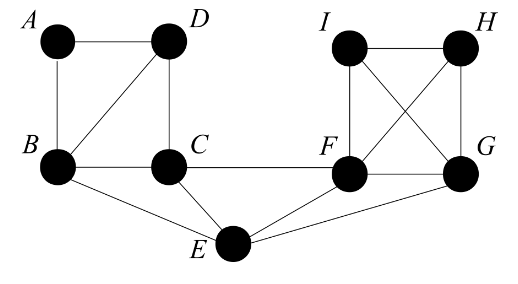
\includegraphics[width=0.6\columnwidth]{img/MCP2}
\end{center}

Start from $x^{(0)} = \{B, C , D\}$, with $w = [\; 0 \; 1 \; 1\; 1\; 0\; 0\; 0\; 0\; 0\; ]$
\begin{enumerate}
	\item $w (\{B, C , E \}) = w (\{A, B, D\}) = 2$, but $\{A, B, D\}$ wins lexicographically: $x^{(1)} = \{A, B, D\}$ with $w = [\; 1\; 2\; 1\; 2\; 0\; 0\; 0\; 0\; 0\; ]$
	
	\item $x^{(2)} = \{B, C , D\}$ with $w = [\; 1\; 3\; 2\; 3\; 0\; 0\; 0\; 0\; 0\; ]$ is the only neighbor
	
	\item $w (\{B, C , E \}) = 5 < 7 = w (\{A, B, D\})$: $x^{(3)} = \{B, C , E \}$ with $w = [\; 1\; 4\; 3\; 3\; 1\; 0\; 0\; 0\; 0\; ]$
	
	\item $w (\{C , E , F \}) = 4 < 10 = w (\{B, C , D\})$: $x^{(4)} = \{C , E , F \}$ with $w = [\; 1\; 4\; 4\; 3\; 2\; 1\; 0\; 0\; 0\; ]$
	
	\item $w (\{E , F , G \}) = 3 < 11 = w (\{B, C , E \})$: $x^{(5)} = \{E , F , G \}$ with $w = [\; 1\; 4\; 4\; 3\; 3\; 2\; 1\; 0\; 0\; ]$
	
	\item $w (\{F , G , H\}) = w (\{F , G , I \}) = 3 < 9 = w (\{C , E , F \})$: $x^{(6)} = \{F , G , H\}$ with $w = [\; 1\; 4\; 4\; 3\; 3\; 3\; 2\; 1\; 0\; ]$
\end{enumerate}

Now the neighborhood $N_{\mathcal{A}_1}$ is not empty: $x^{(7)} = \{F , G , H, I \}$

\newpage

\paragraph{Example:} DLS for the MAX-SAT. Given $m$ logical disjunctions depending on $n$ logical variables, find a truth assignment satisfying the maximum number of clauses
\begin{itemize}
	\item Neighborhood $N_{\mathcal{F}_1}$ (1-flip) is generated complementing a variable.\\
	
	\item Associate to each logical clause a penalty $w_j$ initially equal to $1$ (each component is a satisfied formula).\\
	
	\item The exchange heuristic maximizes the weight of satisfied clauses thus modifying their number with the multiplicative penalty.\\
	
	\item The penalty is updated
	\begin{enumerate}
		\item increasing the weight of unsatisfied clauses to favor them
		$$ w_j := \alpha_{us} w_j \text{ for each } j \in U (x) \; (\text{with } \alpha_{us} > 1) $$
		when a local optimum is reached
		
		\item reducing the penalty towards 1
		$$ w_j := (1 - \rho) w_j + \rho \cdot 1 \text{ for each } j \in C (\text{with } \rho \in (0, 1)) $$
		with a certain probability or after a certain number of updates
	\end{enumerate}
\end{itemize}

The rationale of the method consists in aiming to
\begin{itemize}
	\item satisfy the currently unsatisfied clauses (diversification)
	
	\item in particular, those which have been unsatisfied for longer time and more recently (memory)
\end{itemize}

The parameters tune intensification and diversification
\begin{itemize}
	\item small values of $\alpha_{us}$ and $\rho$ preserve the current penalty (intensification)
	
	\item large values of $\alpha_{us}$ push away from the current solution (diversification)
	
	\item large values of $\rho$ lead push towards the local optimum of the current attraction basin (a different kind of intensification)
\end{itemize}

% End of L18

\newpage

\subsection{Extending the local search with worsenings}

If the neighborhood and objective remain the same, the rule of acceptance must change: instead of
$$ x' := \arg \min_{x\in N(x)} f (x) $$
\textbf{select a nonminimal (possibly, even non-improving) solution}.\\

The main problem is the \textbf{risk of cyclically visiting the same solutions}.\\

The two main strategies that allow to control this risk are
\begin{itemize}
	\item \textbf{Simulated Annealing} (SA), which uses \textbf{randomization} to make repetitions unlikely.\\
	
	\item \textbf{Tabu Search} (TS), which uses \textbf{memory} to forbid repetitions.\\
\end{itemize}

\newpage

\subsection{Simulated Annealing}

The SA derives from Metropolis' algorithm (1953), which aims to simulate the "annealing" process of metals:
\begin{itemize}
	\item bring the metal to a temperature close to fusion, so that its particles distribute at random
	
	\item cool the metal very slowly, so that the energy decreases, but in a time sufficiently long to converge to thermal equilibrium (all the parts cool down equally, so the particles should diffuse equally)
\end{itemize}

The aim of the process is to obtain
\begin{itemize}
	\item a very regular and defectless crystal lattice, that corresponds to the base state (minimum energy configuration)
	
	\item a material with useful physical properties
\end{itemize}

The situation has \textbf{similarities with Combinatorial Optimization problems}
\begin{itemize}
	\item the \textbf{states} of the physical system correspond to the \textbf{solutions}
	
	\item the \textbf{energy} corresponds to the \textbf{objective function}
	
	\item the \textbf{base state} corresponds to the \textbf{globally optimal solutions} (minima)
	
	\item the \textbf{state transitions} correspond to \textbf{local search moves}
	
	\item the \textbf{temperature} corresponds to a \textbf{numerical parameter}
\end{itemize}

This suggests to \textbf{use Metropolis' algorithm for optimization}.\\

According to thermodynamics at the thermal equilibrium the probability of observing each state $i$ depends on its energy $E_i$
$$ \pi'_T (i) = \frac{e^{\frac{-E_i}{k T}}}{\sum_{j \in S} e^{\frac{-E_j}{k t}}}  $$
where $S$ is the state set, $T$ the temperature and $k$ Boltzmann's constant.\\

It is a dynamic equilibrium, with ongoing state transitions in all directions.\\

\newpage

Metropolis' algorithm generates a \textbf{random sequence of states}
\begin{itemize}
	\item the \textbf{current state} $i$ \textbf{has energy} $E_i$
	
	\item the algorithm \textbf{perturbs} $i$, \textbf{generating a state} $j$ \textbf{with energy} $E_j$
	
	\item the \textbf{current state moves from} $i$ \textbf{to} $j$ \textbf{with probability}
	$$ \pi_T (i,j) = \begin{cases}
		1 & \text{ if } E_j < E_i \\
		e^{\frac{E_i - E_j}{k T}} = \frac{\pi' (j)}{\pi' (i)} & \text{ if } E_j \geq E_i \\
	\end{cases} $$
\end{itemize}

that is the transition is
\begin{itemize}
	\item \textbf{Deterministic if improving} (because that is the final purpose, if it's lower, and thus better, go to it).\\
	
	\item \textbf{Based on the conditional probability if worsening} (ratio of the probability of the final state and the probability of the original state); the probability is proportional to how much worse the state is, it it worsens only a little the probability can still be quite big.\\
\end{itemize}

The probability of being in the new state $j$ is equal to the product of the probability of being in the old state $i$ times the probability of the transition.\\

Simulated Annealing applies exactly the same principle.\\

\newpage

\begin{algorithm}
	\caption{Algorithm $SimulatedAnnealing(I , x^{(0)}, T^{[0]})$}
	\begin{algorithmic}
		\STATE $x := x^{(0)}$ 
		\STATE $x^\ast := x^{(0)}$ 
		\STATE $T := T^{[0]}$
		\WHILE{$Stop() = false$}
		\STATE $x' := RandomExtract(N, x)$ // random uniform extraction
		\IF{$f (x') < f (x)$ or $U [0; 1] \leq e^{\frac{f(x) - f(x')}{T}}$} 
		\STATE $x := x'$
		\ENDIF
		\IF{$f (x') < f (x^\ast)$} 
		\STATE $x^\ast := x'$
		\ENDIF
		$T := Update(T )$
		\ENDWHILE
		\RETURN $(x^\ast, f (x^\ast))$
	\end{algorithmic}
\end{algorithm}

As the neighborhood is used to generate a solution (not fully explored), \textbf{it is possible to worsen even if improving solutions exist}.\\

A \textbf{pre-computed table of values for} $e^{\frac{\delta f}{T}}$ \textbf{can improve the efficiency}; they're real numbers so it can't be fully complete, but it's a random rule so does it really matter if it's approximated?.\\

\textbf{Several update schemes} can be designed \textbf{for the "temperature"} $T$.\\

At each step you extract a random solution from the current neighborhood, if it's better than the old one swap them, if it's worse swap them with a certain probability (given by the extraction of a number between 0 and 1 and checking if it's under the value of the formula).\\
Check if the solution is better than the best one.\\
Update $T$, change the value of the temperature, you're simulating an annealing process in which the temperature decreases.\\

Accepting a random value from the neighborhood means that there could be a better solution in the neighborhood.\\
Since there's no exploration, just extracting a random number, the single steps are very fast, but it could require many more steps.

\newpage

\subsubsection{Acceptance criteria}
$T$ rules the \textbf{probability to accept worsenings}
$$ \pi_T (x, x') = \begin{cases}
	1 & \text{ if } f(x') < f(x) \\
	e^{\frac{f(x) - f(x')}{T}} & \text{ if } f(x') \geq f(x)
\end{cases}$$

\begin{itemize}
	\item $T \gg 0$ \textbf{diversifies} because nearly all solutions are accepted: in the extreme case, it is a random walk
	
	\item $T \approx 0$ \textbf{intensifies} nearly all worsening solutions are rejected: in the extreme case, it is a steepest descent
	
\end{itemize}

\begin{center}
	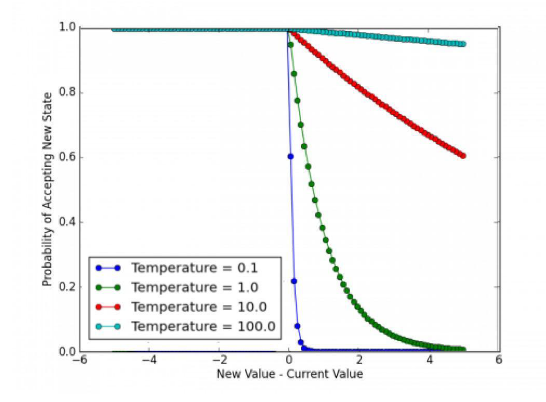
\includegraphics[width=0.6\columnwidth]{img/temp1}
\end{center}

Notice the similarity with the ILS.\\

If you're improving you always accept, if not you accept with a probability based on temperature, the higher the temperature the more the probability to accept the solution increases.\\

\newpage

\subsubsection{Asymptotic convergence to the optimum}

Due to the acceptance rule, \textbf{the current solution} $x$ \textbf{is a random variable} (depends on the random seed given): its "\textbf{state probability}" $\pi' (x)$ (associates a value of probability to each solution) \textbf{combines on all possible predecessors} $x^{(t−1)}$ 
\begin{itemize}
	\item the "state probability" $\pi' (x^{(t−1)})$ of the predecessor
	
	\item the \textbf{probability to choose the move from} $x^{(t−1)}$ to $x$, that is \textbf{uniform}
	
	\item the \textbf{probability to accept the move}, that is
	$$ \pi_T \left(x^{(t-1)}, x\right) = \begin{cases}
		1 & \text{ if } f(x) < f \left(x^{(t-1)}\right) \\
		e^{\frac{f\left(x^{(t-1)}\right) - f(x)}{T}} & \text{ if } f(x) \geq f \left(x^{(t-1)}\right) \\
	\end{cases}$$
\end{itemize}

The probability of being in a given solution $x$ in step $t$ is the combination of all the possible probabilities of the previous step, combined with the probability of choosing that specific solution from the previous step (uniform probability, it's random) and the probability of accepting said solution (stated in the formula).\\

As it \textbf{depends only on the previous step}, the solution is a \textbf{Markov chain}.\\

For fixed temperature $T$, the \textbf{transition probabilities are stationary}: it is a \textbf{homogeneous Markov chain}.\\

If the search graph for neighborhood $N$ is connected, the \textbf{probability to reach each state is} $> 0$: it is an \textbf{irreducible Markov chain}.\\

Under these assumptions (irreducible and homogeneous Markov chain), \textbf{the state probability converges to a stationary distribution independent of the starting state}. \\
For any starting state, the probability of being in a given solution after a long time tends to assume a stationary distribution, i.e. the behavior of the algorithm is not influenced by the starting solution.\\

%\newpage

The stationary distribution favors "good" solutions with the same law imposed by thermodynamics on physical systems at thermal equilibrium
$$ \pi_T (x) = \frac{ e^{\frac{-f(x)}{T}} }{ \sum_{x \in X} e^{\frac{-f(x)}{T}} } \text{ for each } x \in X $$

where $X$ is the feasible region and $T$ the "temperature" parameter-\\

The \textbf{distribution converges} to a \textbf{limit distribution} as $T \rightarrow 0$
$$ \pi (x) = \lim_{T \rightarrow 0} \pi_T (x) = \begin{cases}
	\frac{1}{|X^\ast|} & \text{ for } x \in X^\ast \\
	0 & \text{ for } x \in X \setminus X^\ast\\
\end{cases}$$
which corresponds to a \textbf{certain convergence to a globally optimal solution}.\\

This result however holds at the equilibrium, in infinite time.\\

In practice, \textbf{low values of} $T$ imply
\begin{itemize}
	\item a \textbf{high probability to visit a global optimum}, but also
	\item a \textbf{slow convergence} to the optimum (many exchanges are rejected)
\end{itemize}

In a finite time, the result obtained with \textbf{low} $T$ can be \textbf{far from optimal}.\\
Hence, $T$ \textbf{starts high} and is progressively updated \textbf{decreasing over time}.\\

The \textbf{starting value} $T^{[0]}$ should be
\begin{itemize}
	\item \textbf{high enough} to allow to \textbf{reach any solution quickly}
	\item \textbf{small enough} to \textbf{discourage visiting very bad solutions}
\end{itemize}

A classical tuning for $T^{[0]}$ is to
\begin{itemize}
	\item sample the first neighborhood $N (x^{(0)})$
	\item set a parameter $\beta \in (0, 1)$
	\item set $T^{[0]}$ to accept on average a fraction $\beta$ of the sampled solutions
\end{itemize}

\newpage

\subsubsection{Temperature update}
The temperature is \textbf{updated by subsequent phases} $(r = 0, \, ... \, , m)$
\begin{itemize}
	\item \textbf{each phase} applies a \textbf{constant value} $T^{[r]}$ \textbf{for} $\ell^{[r ]}$ iterations
	
	\item $T^{[r]}$ \textbf{decreases exponentially from phase to phase}
	$$ T^{[r ]} := \alpha T^{[r −1]} = \alpha^r T^{[0]} \text{ with } \alpha \in (0, 1) $$
	
	\item $\ell^{[r ]}$ \textbf{increases from phase to phase} (often linearly) \textbf{with values related to the diameter of the search graph} (therefore to the size of the instance)
\end{itemize}

Since $T$ is variable, the Markov chain $x$ is not homogeneous, but
\begin{itemize}
	\item if $T$ \textbf{decreases slowly enough}, it \textbf{converges to the global optimum}
	
	\item \textbf{good parameters} to tune the decrease \textbf{depend on the instance} (namely, on $f (\tilde{x}) - f (x^\ast)$, where $f (\tilde{x})$ is the second best value of $f$; but the best parameter values are not known a priori)
\end{itemize}

\textbf{Adaptive SA} variants \textbf{tune the temperature} $T$ \textbf{based on the results}
\begin{itemize}
	\item \textbf{set} $T$ to a value such that a given \textbf{fraction of} $N (x)$ is \textbf{accepted}
	
	\item \textbf{increase} $T$ if the \textbf{solution has not improved for a certain time} (diversification); \textbf{otherwise decrease it} (intensification)
\end{itemize}

\newpage

\subsection{Tabu Search}
The Tabu Search (TS) has been proposed by Glover (1986).\\

It keeps the basic selection rule of steepest descent
$$ x' := \arg \min_{x \in N(x)} f (x) $$

\textbf{without the termination condition} (but this implies cycling!).\\

The TS imposes a tabu to \textbf{forbid the solutions already visited}
$$ x' := \arg \min_{x \in N(x) \setminus X_V} f(x) $$

where $X_V$ is the set of the already visited solutions.\\

\paragraph{Exchange heuristics with tabu:} An exchange heuristic that explores a neighborhood imposing a tabu on the already visited solutions requires to:
\begin{enumerate}
	\item \textbf{evaluate the feasibility} of each subset produced by the exchanges (unless guaranteed a priori)
	
	\item \textbf{evaluate the cost} of each feasible solution
	
	\item \textbf{evaluate the tabu status} of each feasible promising solution
	
\end{enumerate}
in order to \textbf{select the feasible best non-tabu solution}.\\

An elementary way to implement the evaluation of the tabu is
\begin{itemize}
	\item save the visited solutions in a suitable structure (tabu list)
	\item check each explored solution making a query on the tabu list
\end{itemize}

\newpage

\paragraph{Potential inefficiency of the tabu mechanism:} This elementary evaluation of the tabu however is \textbf{very inefficient}
\begin{itemize}
	\item the \textbf{comparison of the solutions} at step $t$ requires \textbf{time} $O (t)$ (reducible with hash tables or search trees)
	\item the \textbf{number of solutions} visited \textbf{grows indefinitely} over time
	\item the \textbf{memory occupation grows indefinitely} over time
\end{itemize}

The \textit{Cancellation Sequence Method} and the \textit{Reverse Elimination Method} tackle these problems, exploiting the fact that in general
\begin{itemize}
	\item the \textbf{solutions visited} form a \textbf{chain with small variations}
	\item the \textbf{solutions visited} are \textbf{rarely neighbors} of the \textbf{current one}
\end{itemize}

The idea is to \textbf{focus on variations}
\begin{itemize}
	\item \textbf{save move lists}, instead of solutions
	\item \textbf{evaluate} the \textbf{overall performed variations}, instead of the single moves
	\item \textbf{find the solutions which have undergone small overall variations} (recent ones or submitted to variations subsequently reversed)
\end{itemize}

\vfill

\paragraph{Potential ineffectiveness of the tabu mechanism:} Other subtle phenomena influence the \textbf{effectiveness of the method}.\\

\textbf{Forbidding the solutions visited} can have two different \textbf{negative effects}:
\begin{itemize}
	\item it can \textbf{disconnect the search graph}, creating impassable "iron curtains" that block the search (the prohibition should not be permanent)
	
	\item it can \textbf{slow down the exit from attraction basins}, creating a "gradual filling" effect that slows down the search (the prohibition should be extended)
\end{itemize}

The two phenomena suggest apparently opposite remedies. How to combine them? \\

\newpage

\subsubsection{Reducing potential ineffectiveness}

Some simple devices can be adopted in order to control these problems.\\

\paragraph{Attribute-based tabu:} Forbid all \textbf{solutions that share "attributes" with the visited ones}.\\

Forbidding only the visited solution slows down the search, so instead
\begin{itemize}
	\item define a \textbf{set} $A$ \textbf{of attributes} (general attributes that any solution can have)
	
	\item define \textbf{for each solution} $x \in X$ a \textbf{subset of attributes} $A_x \subseteq A$ (what attributes does each solution have)
	
	\item declare a \textbf{subset of tabu attributes} $\overline{A} \subseteq A$ (empty at first; what attributes are forbidden)
	
	\item \textbf{forbid} all the \textbf{solutions with tabu attributes}
	$$ x \text{ is tabu } \Leftrightarrow A_x \cap \overline{A} \neq \emptyset $$
	(if the solution has an attribute inside $\overline{A}$ then forbid it)
	
	\item \textbf{move from} the current solution $x$ \textbf{to} $x'$ such that $A_{x'} \cap \overline{A} = \emptyset$ (the new solution has no forbidden attributes) and add to $\overline{A}$ the attributes possessed by $x$ and not by $x'$
	$$ \overline{A} := \overline{A} \cup (A_x \setminus A{x'} ) $$
	(in this way, $x$ becomes tabu)
\end{itemize}
You don't check a list of tabu solutions, the criteria to forbid a solution is the intersection of its attributes with the set of forbidden ones.\\

This allows to
\begin{itemize}
	\item \textbf{avoid} also \textbf{solutions similar to the visited ones}
	\item \textbf{get} more quickly \textbf{far away from visited local optima}
\end{itemize}

\newpage

The \textbf{concept of "attribute"} is intentionally \textbf{generic}; the simpler ones are
\begin{itemize}
	\item \textbf{Inclusion of an element in the solution} ($A = B$ and $A_x = x$): when the move from $x$ to $x'$ expels an element $i$ from the solution, the tabu forbids the reinsertion of $i$ in the solution
	\begin{itemize}
		\item $x$ has the attribute "presence of $i$" and $x'$ hasn't got it
		\item the attribute "presence of $i$" enters $\overline{A}$
		\item every solution including $i$ becomes tabu
	\end{itemize}
	\nn
	
	\item \textbf{Exclusion of an element from the solution} ($A = B$ and $A_x = B \setminus x$): when the move from $x$ to $x'$ inserts an element $i$ into the solution, the tabu forbids the removal of $i$ from the solution
	\begin{itemize}
		\item $x$ has the attribute "absence of $i$" and $x'$ hasn't got it
		\item the attribute "absence of $i$" enters $\overline{A}$
		\item every solution devoid of $i$ becomes tabu
	\end{itemize}
	\nn
\end{itemize}

\textbf{Different attribute sets can be combined}, each with its tenure and list (e.g., after replacing $i$ with $j$, forbid both to remove $j$ and to insert $i$).\\

Other (less frequent) examples of attributes:
\begin{itemize}
	\item the \textbf{value of the objective function}: forbid solutions of a given value, previously assumed by the objective
	\item the \textbf{value of an auxiliary function}
\end{itemize}

Complex attributes can be obtained combining simple attributes
\begin{itemize}
	\item the \textbf{coexistence} in the solution \textbf{of two elements} (or their separation) 
	\item or, if a move replaces element $i$ with element $j$, the tabu can \textbf{forbid the removal of} $j$ \textbf{to include} $i$, but allow the simple removal of $j$ and the simple inclusion of $i$
\end{itemize}

\newpage

Other solutions:

\paragraph{Give a limited length $L$ (tabu tenure) to the prohibition:} The tabu mechanism creates regions hard or impossible to reach
\begin{itemize}
	\item the \textbf{tabu solutions} become \textbf{feasible again after a while}
	
	\item the \textbf{same solutions can be revisited} (but, if $\overline{A}$ is different, the \textbf{future evolution will be different}, if the evolution is the same you're stuck in a cycle)
\end{itemize}

Tuning the tabu tenure is fundamental for the effectiveness of TS\\

\paragraph{Introduce an aspiration criteria:} The tabu could forbid a global optimum similar to a visited solution, so a tabu solution \textbf{better than the best known} one is anyway \textbf{accepted} (obviously, there is no risk of looping).\\

There are looser aspiration criteria, but they are not commonly used.\\

\paragraph{If all neighbour solutions are tabu, accept the one with the oldest tabu:} The tabu could forbid all neighbour solutions. It can be interpreted as another aspiration criteria.\\
Otherwise the algorithm would just "sit still" and waste time until a tabu expires.\\

\newpage

\subsubsection{General scheme of the TS}

\begin{algorithm}
	\caption{Algorithm $TabuSearch(I , x^{(0)}, L)$}
	\begin{algorithmic}
		\STATE $x := x^{(0)}$ 
		\STATE $x^\ast := x^{(0)}$
		\STATE $\overline{A} := \emptyset$
		\WHILE{$Stop() = false$}
		\STATE $f' := + \infty$
		\FOR{each $y \in N (x)$}
		\IF{$f (y ) < f'$}
		\IF{$Tabu(y , \overline{A}) = false$ or $f(y) < f (x^\ast)$} 
		\STATE $x' := y$
		\STATE $f' := f (y )$
		\ENDIF
		\ENDIF
		\ENDFOR
		\STATE $\overline{A} := Update( \overline{A}, x', L)$
		\IF{$f (x') < f (x^\ast)$} 
		\STATE $x^\ast := x'$
		\ENDIF
		\ENDWHILE
		\RETURN $(x^\ast, f (x^\ast))$
	\end{algorithmic}
\end{algorithm}

Until the termination condition holds, for each neighbor solution finds which one is the best one; if they're not tabu or if they meet the aspiration criteria, they become the new chosen solution.\\
After every inner loop it updates the tabu list with the elements of the new solution found and the tenure of already forbidden elements (represented with $L$).\\

\newpage

\subsubsection{Efficient evaluation of the tabu status}

The \textbf{evaluation} of the tabu status must be \textbf{efficient} and avoid scanning the whole solution (as for feasibility and cost)
\begin{itemize}
	\item the \textbf{attributes are associated to moves, not to solutions}: do not check whether the solution includes $i$, but whether the move adds $i$
\end{itemize}

Let $T_i$ be the iteration when attribute $i \in A$ became tabu ($-\infty$ if $i \notin \overline{A}$).\\

To \textbf{evaluate} the tabu status in \textbf{constant time} simply \textbf{check}
$$ t \leq T_i + L $$

If the tabu is on insertions $(A = x)$, at iteration $t$
\begin{itemize}
	\item forbid the moves that add $i \in B \setminus x$ when $t \leq T_i^{in} + L^{in}$
	
	\item update $T_i^{in} := t$ for each $i$ removed $(i \in x \setminus x')$
\end{itemize}

If the tabu is on deletions $(A = B \setminus x)$, at iteration $t$
\begin{itemize}
	\item forbid the moves that delete $i \in x$ when $t \leq T_i^{out} + L^{out}$
	
	\item update $T_i^{out} := t$ for each $i$ added $(i \in x' \setminus x)$
\end{itemize}

As either $i \in x$ or $i \in B \setminus x$, \textbf{a single vector} $T$ \textbf{is enough for both checks} (an element can either be in or out).\\

More sophisticated attributes require more complex structures.\\

\newpage

\paragraph{Example:} the TSP. Consider the neighborhood $N_{\mathcal{R}_2}$ generated by 2-opt exchanges and use as attributes both the presence and the absence of arcs in the solution
\begin{itemize}
	\item At first set $T_{ij} = -\infty$ for each arc $(i, j) \in A$.\\
	
	\item At each step $t$, explore the $n(n − 1)/2$ pairs of removable arcs and the corresponding pairs of arcs which would replace them.\\
	
	\item The move $(i, j)$, which replaces $(s_i , s_{i+1})$ and $(s_j , s_{j+1})$ with $(s_i , s_j )$ and $(s_{i+1}, s_{j+1})$, is tabu at step $t$ if one of the following conditions holds:
	\begin{enumerate}
		\item $t \leq T_{s_i ,s_{i+1}} + L^{out}$
		\item $t \leq T_{s_j ,s_{j+1}} + L^{out}$
		\item $t \leq T_{s_i ,s_j} + L^{in}$
		\item $t \leq T_{s_{j+1},s_{i+1}} + L^{in}$
	\end{enumerate}
	So, at first all moves are legal. This is basically checking if all the addition and deletion moves respect the tabu conditions; check when the arcs to add were expelled and when the arcs to remove were added, and if it's long enough ago (possibly never) they are not tabu (the value $+$ tenure must be lower than $t$).\\
	If any of these conditions holds, one of the elements is tabu and the move is forbidden.\\
	
	\item For the selected move $(i^\ast, j^\ast$), update the auxiliary structures setting
	\begin{enumerate}
		\item $T_{s_{i^\ast} ,s_{i^\ast + 1}} := t$
		\item $T_{s_{j^\ast} ,s_{j^\ast + 1}} := t$
		\item $T_{s_{i^\ast} ,s_{j^\ast}} := t$
		\item $T_{s_{j^\ast + 1},s_{i^\ast + 1}} := t$
	\end{enumerate}
	Set the value of $T$ to the number of the current iteration for the affected arcs.\\
\end{itemize}

As $n$ arcs are in and $n(n − 2)$ out of the solution, it is better to set $L^{out} \ll L^{in}$. This also holds for every problem in which the solution is much smaller than the ground set (often).\\

\newpage

\paragraph{Example:} the Max-SAT. Consider the neighborhood $N_{\mathcal{F}_1}$, which includes the solutions obtained complementing the value of a variable (all $n$ solutions are feasible; one flip neighborhood).\\

Since $|x| = |B \setminus x|$ for each $x \in X$ (the number of elements in the solution are the same as the number of elements outside)
\begin{itemize}
	\item the tabu tenure for additions and deletions can be the same
	
	\item it is sufficient to forbid the change of value of a variable and the attribute is the variable
\end{itemize}

The algorithm proceeds as follows
\begin{itemize}
	\item At first, set $T_i = -\infty$ for each variable $i = 1,\, ... \, , n$.\\
	
	\item at each step $t$, explore the $n$ solutions obtained complementing each variable.\\
	
	\item the move $i$, which assigns $x_i := \overline{x}_i$ (flips the variable), is tabu at step $t$ if $t \leq T_i + L$ (it needs to be long enough since the variable has last been flipped; at first all moves are non-tabu).\\
	
	\item perform move $i^\ast$ and set $T_{i^\ast} := t$.\\
\end{itemize}

\newpage

\subsubsection{Tuning the tabu tenure}
The value of the tabu tenure $L$ is a \textbf{crucial parameter}
\begin{itemize}
	\item \textbf{too large} tenures can \textbf{conceal the global optimum} and in the worst case \textbf{block the search}
	
	\item \textbf{too small} tenures can \textbf{hold the exploration back in useless regions} and in the worst case \textbf{produce cyclic behaviors}
\end{itemize}
\nn

The \textbf{most effective value} of $L$ is in general
\begin{itemize}
	\item \textbf{related} to the \textbf{size of the instance} (big instances require more prohibition)
	
	\item \textbf{slowly growing with size} (many authors suggest $L \in O(\sqrt{|A|})$, the value of tenure grows with the square root of the value of attributes)
	
	\item but nearly \textbf{constant on medium ranges of size} (if the size doesn't change very much there's no need to change the tenure)
\end{itemize}

\textbf{Cycles can be broken} extracting $L$ at \textbf{random in a range} $[L_{min}; L_{max}]$.\\

\nn
\textbf{Adaptive mechanisms} update $L$ \textbf{based on the results} of the search within a given range $[L_{min}; L_{max}]$
\begin{itemize}
	\item \textbf{decrease} $L$ when the \textbf{current solution} $x$ \textbf{improves}: the search is probably approaching a new local optimum, and we want to favor it (intensification)
	
	\item \textbf{increase} $L$ when the \textbf{current solution} $x$ \textbf{worsens}: the search is probably leaving a known local optimum, and we want to speed up (diversification)
\end{itemize}

\newpage

\subsubsection{Variants}

Other adaptive strategies work in the long term:
\begin{itemize}
	\item \textbf{Reactive Tabu Search:}
	\begin{itemize}
		\item use efficient structures to save the solutions visited (hash table)
		\item detect cyclic behaviors (frequent repetitions)
		\item move the range $[L_{min}; L_{max}]$ upwards if the solutions repeat too often
	\end{itemize}
	\nn
	
	\item \textbf{Frequency-based Tabu Search:}
	\begin{itemize}
		\item save the frequency of each attribute in the solution in structures similar to the ones used for the tenure (e.g., $F_i$ for each $i \in B$)
		\item if an attribute appears very often
		\begin{itemize}
			\item favor the moves introducing it modifying $f$ as in the DLS
			\item forbid the moves introducing it, or discourage them by modifying $f$
		\end{itemize}
	\end{itemize}
	\nn
	
	\item \textbf{Exploring Tabu Search:} reinitialize the search from solutions of good quality which have been explored, but not used as current solution (i. e., the "second-best solutions" of some neighborhood).\\
	
	\item \textbf{Granular Tabu Search:} enlarge or reduce the neighborhood progressively.\\
\end{itemize}

% End of L19, L20 is lab, L21 from here

\newpage